% Created by tikzDevice version 0.12.4 on 2023-07-19 22:10:04
% !TEX encoding = UTF-8 Unicode
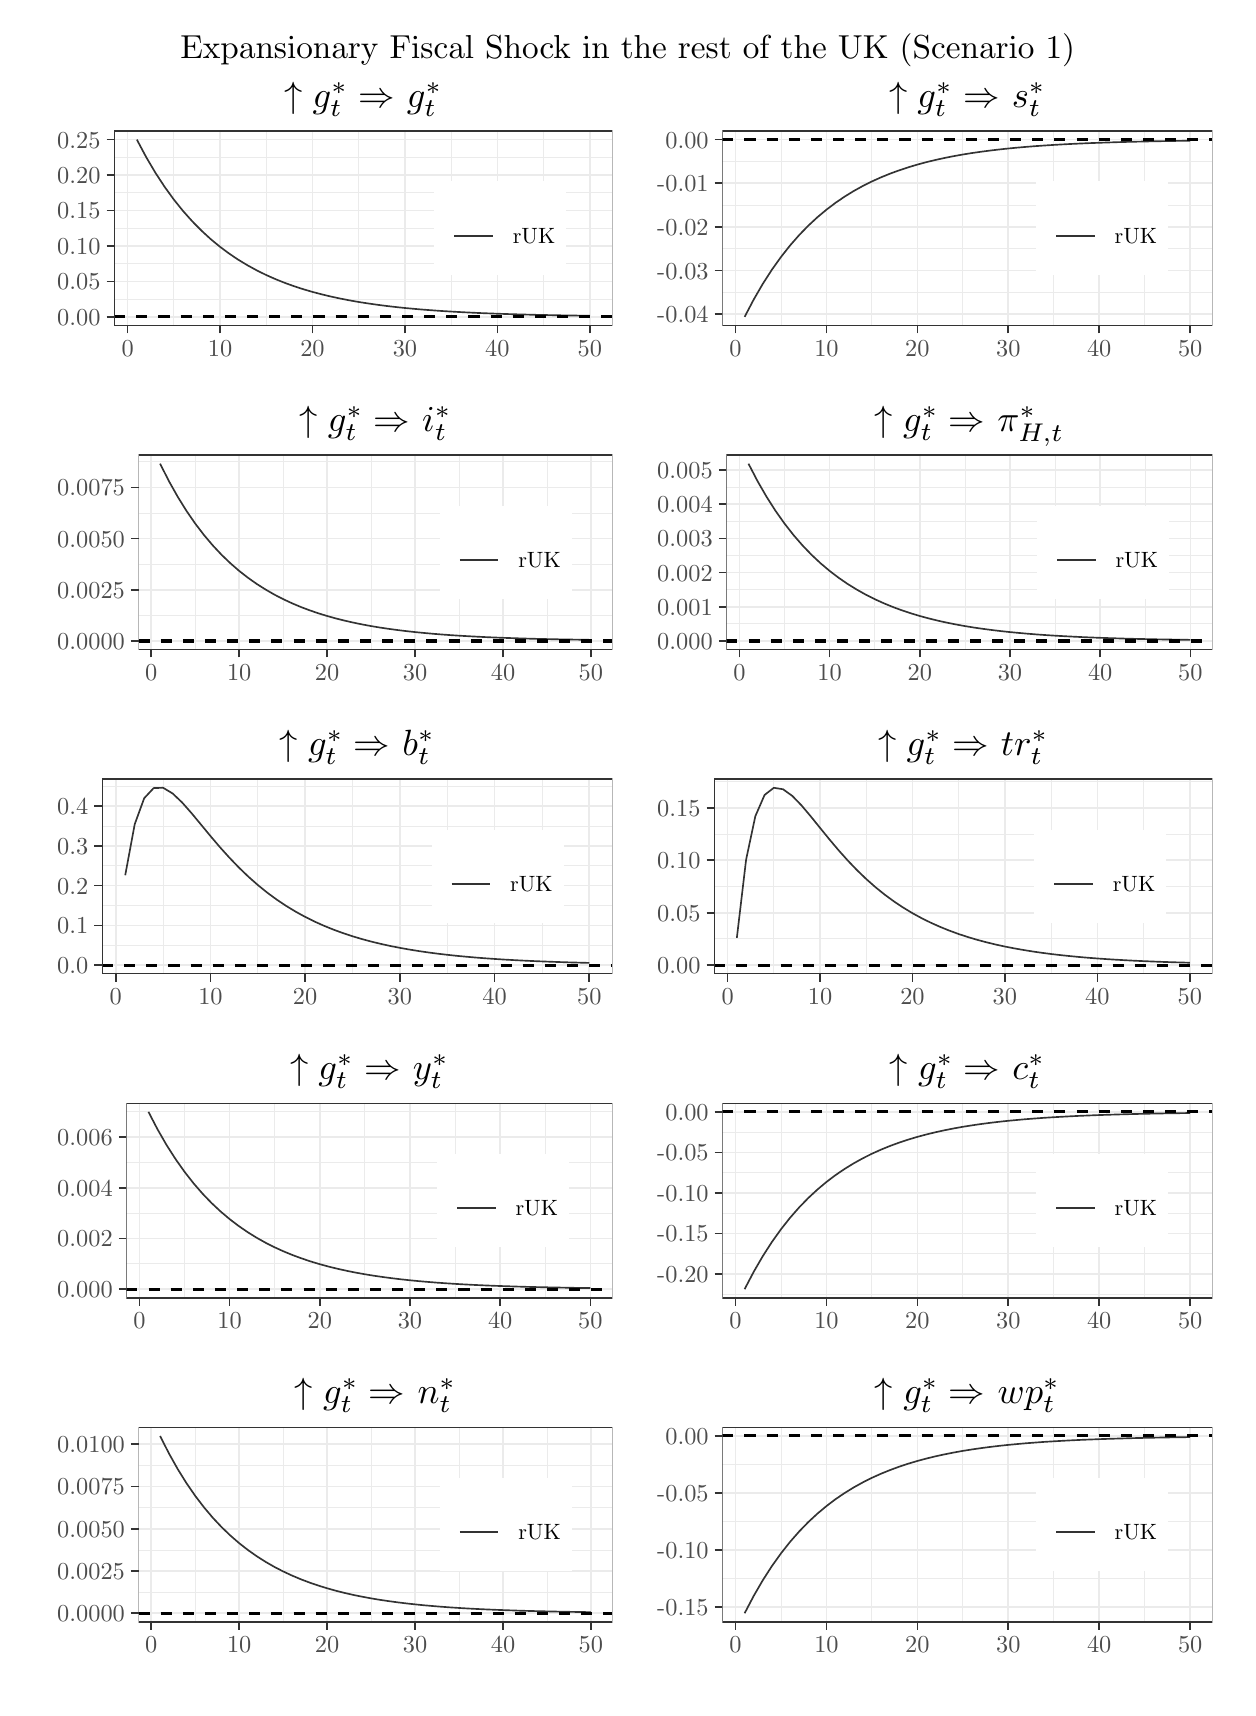
\begin{tikzpicture}[x=1pt,y=1pt]
\definecolor{fillColor}{RGB}{255,255,255}
\path[use as bounding box,fill=fillColor,fill opacity=0.00] (0,0) rectangle (433.62,599.84);
\begin{scope}
\path[clip] (  0.00,468.44) rectangle (216.81,585.55);
\definecolor{drawColor}{RGB}{255,255,255}
\definecolor{fillColor}{RGB}{255,255,255}

\path[draw=drawColor,line width= 0.6pt,line join=round,line cap=round,fill=fillColor] (  0.00,468.44) rectangle (216.81,585.55);
\end{scope}
\begin{scope}
\path[clip] ( 31.27,492.12) rectangle (211.31,562.59);
\definecolor{fillColor}{RGB}{255,255,255}

\path[fill=fillColor] ( 31.27,492.12) rectangle (211.31,562.59);
\definecolor{drawColor}{gray}{0.92}

\path[draw=drawColor,line width= 0.3pt,line join=round] ( 31.27,501.73) --
	(211.31,501.73);

\path[draw=drawColor,line width= 0.3pt,line join=round] ( 31.27,514.54) --
	(211.31,514.54);

\path[draw=drawColor,line width= 0.3pt,line join=round] ( 31.27,527.36) --
	(211.31,527.36);

\path[draw=drawColor,line width= 0.3pt,line join=round] ( 31.27,540.17) --
	(211.31,540.17);

\path[draw=drawColor,line width= 0.3pt,line join=round] ( 31.27,552.98) --
	(211.31,552.98);

\path[draw=drawColor,line width= 0.3pt,line join=round] ( 52.81,492.12) --
	( 52.81,562.59);

\path[draw=drawColor,line width= 0.3pt,line join=round] ( 86.22,492.12) --
	( 86.22,562.59);

\path[draw=drawColor,line width= 0.3pt,line join=round] (119.62,492.12) --
	(119.62,562.59);

\path[draw=drawColor,line width= 0.3pt,line join=round] (153.02,492.12) --
	(153.02,562.59);

\path[draw=drawColor,line width= 0.3pt,line join=round] (186.43,492.12) --
	(186.43,562.59);

\path[draw=drawColor,line width= 0.6pt,line join=round] ( 31.27,495.32) --
	(211.31,495.32);

\path[draw=drawColor,line width= 0.6pt,line join=round] ( 31.27,508.14) --
	(211.31,508.14);

\path[draw=drawColor,line width= 0.6pt,line join=round] ( 31.27,520.95) --
	(211.31,520.95);

\path[draw=drawColor,line width= 0.6pt,line join=round] ( 31.27,533.76) --
	(211.31,533.76);

\path[draw=drawColor,line width= 0.6pt,line join=round] ( 31.27,546.58) --
	(211.31,546.58);

\path[draw=drawColor,line width= 0.6pt,line join=round] ( 31.27,559.39) --
	(211.31,559.39);

\path[draw=drawColor,line width= 0.6pt,line join=round] ( 36.11,492.12) --
	( 36.11,562.59);

\path[draw=drawColor,line width= 0.6pt,line join=round] ( 69.52,492.12) --
	( 69.52,562.59);

\path[draw=drawColor,line width= 0.6pt,line join=round] (102.92,492.12) --
	(102.92,562.59);

\path[draw=drawColor,line width= 0.6pt,line join=round] (136.32,492.12) --
	(136.32,562.59);

\path[draw=drawColor,line width= 0.6pt,line join=round] (169.72,492.12) --
	(169.72,562.59);

\path[draw=drawColor,line width= 0.6pt,line join=round] (203.13,492.12) --
	(203.13,562.59);
\definecolor{drawColor}{gray}{0.20}

\path[draw=drawColor,line width= 0.6pt,line join=round] ( 39.45,559.39) --
	( 42.79,553.11) --
	( 46.13,547.45) --
	( 49.47,542.34) --
	( 52.81,537.73) --
	( 56.15,533.58) --
	( 59.50,529.83) --
	( 62.84,526.45) --
	( 66.18,523.39) --
	( 69.52,520.64) --
	( 72.86,518.16) --
	( 76.20,515.92) --
	( 79.54,513.91) --
	( 82.88,512.08) --
	( 86.22,510.44) --
	( 89.56,508.96) --
	( 92.90,507.62) --
	( 96.24,506.42) --
	( 99.58,505.33) --
	(102.92,504.35) --
	(106.26,503.47) --
	(109.60,502.67) --
	(112.94,501.95) --
	(116.28,501.30) --
	(119.62,500.71) --
	(122.96,500.19) --
	(126.30,499.71) --
	(129.64,499.28) --
	(132.98,498.89) --
	(136.32,498.54) --
	(139.66,498.23) --
	(143.00,497.94) --
	(146.34,497.69) --
	(149.68,497.45) --
	(153.02,497.25) --
	(156.36,497.06) --
	(159.70,496.89) --
	(163.04,496.73) --
	(166.38,496.60) --
	(169.72,496.47) --
	(173.06,496.36) --
	(176.40,496.26) --
	(179.74,496.17) --
	(183.08,496.08) --
	(186.43,496.01) --
	(189.77,495.94) --
	(193.11,495.88) --
	(196.45,495.83) --
	(199.79,495.78) --
	(203.13,495.73);
\definecolor{drawColor}{RGB}{0,0,0}

\path[draw=drawColor,line width= 1.1pt,dash pattern=on 4pt off 4pt ,line join=round] ( 31.27,495.32) -- (211.31,495.32);
\definecolor{drawColor}{gray}{0.20}

\path[draw=drawColor,line width= 0.6pt,line join=round,line cap=round] ( 31.27,492.12) rectangle (211.31,562.59);
\end{scope}
\begin{scope}
\path[clip] (  0.00,  0.00) rectangle (433.62,599.84);
\definecolor{drawColor}{gray}{0.30}

\node[text=drawColor,anchor=base east,inner sep=0pt, outer sep=0pt, scale=  0.88] at ( 26.32,492.29) {0.00};

\node[text=drawColor,anchor=base east,inner sep=0pt, outer sep=0pt, scale=  0.88] at ( 26.32,505.11) {0.05};

\node[text=drawColor,anchor=base east,inner sep=0pt, outer sep=0pt, scale=  0.88] at ( 26.32,517.92) {0.10};

\node[text=drawColor,anchor=base east,inner sep=0pt, outer sep=0pt, scale=  0.88] at ( 26.32,530.73) {0.15};

\node[text=drawColor,anchor=base east,inner sep=0pt, outer sep=0pt, scale=  0.88] at ( 26.32,543.55) {0.20};

\node[text=drawColor,anchor=base east,inner sep=0pt, outer sep=0pt, scale=  0.88] at ( 26.32,556.36) {0.25};
\end{scope}
\begin{scope}
\path[clip] (  0.00,  0.00) rectangle (433.62,599.84);
\definecolor{drawColor}{gray}{0.20}

\path[draw=drawColor,line width= 0.6pt,line join=round] ( 28.52,495.32) --
	( 31.27,495.32);

\path[draw=drawColor,line width= 0.6pt,line join=round] ( 28.52,508.14) --
	( 31.27,508.14);

\path[draw=drawColor,line width= 0.6pt,line join=round] ( 28.52,520.95) --
	( 31.27,520.95);

\path[draw=drawColor,line width= 0.6pt,line join=round] ( 28.52,533.76) --
	( 31.27,533.76);

\path[draw=drawColor,line width= 0.6pt,line join=round] ( 28.52,546.58) --
	( 31.27,546.58);

\path[draw=drawColor,line width= 0.6pt,line join=round] ( 28.52,559.39) --
	( 31.27,559.39);
\end{scope}
\begin{scope}
\path[clip] (  0.00,  0.00) rectangle (433.62,599.84);
\definecolor{drawColor}{gray}{0.20}

\path[draw=drawColor,line width= 0.6pt,line join=round] ( 36.11,489.37) --
	( 36.11,492.12);

\path[draw=drawColor,line width= 0.6pt,line join=round] ( 69.52,489.37) --
	( 69.52,492.12);

\path[draw=drawColor,line width= 0.6pt,line join=round] (102.92,489.37) --
	(102.92,492.12);

\path[draw=drawColor,line width= 0.6pt,line join=round] (136.32,489.37) --
	(136.32,492.12);

\path[draw=drawColor,line width= 0.6pt,line join=round] (169.72,489.37) --
	(169.72,492.12);

\path[draw=drawColor,line width= 0.6pt,line join=round] (203.13,489.37) --
	(203.13,492.12);
\end{scope}
\begin{scope}
\path[clip] (  0.00,  0.00) rectangle (433.62,599.84);
\definecolor{drawColor}{gray}{0.30}

\node[text=drawColor,anchor=base,inner sep=0pt, outer sep=0pt, scale=  0.88] at ( 36.11,481.11) {0};

\node[text=drawColor,anchor=base,inner sep=0pt, outer sep=0pt, scale=  0.88] at ( 69.52,481.11) {10};

\node[text=drawColor,anchor=base,inner sep=0pt, outer sep=0pt, scale=  0.88] at (102.92,481.11) {20};

\node[text=drawColor,anchor=base,inner sep=0pt, outer sep=0pt, scale=  0.88] at (136.32,481.11) {30};

\node[text=drawColor,anchor=base,inner sep=0pt, outer sep=0pt, scale=  0.88] at (169.72,481.11) {40};

\node[text=drawColor,anchor=base,inner sep=0pt, outer sep=0pt, scale=  0.88] at (203.13,481.11) {50};
\end{scope}
\begin{scope}
\path[clip] (  0.00,  0.00) rectangle (433.62,599.84);
\definecolor{fillColor}{RGB}{255,255,255}

\path[fill=fillColor] (146.96,510.43) rectangle (194.64,544.28);
\end{scope}
\begin{scope}
\path[clip] (  0.00,  0.00) rectangle (433.62,599.84);
\definecolor{fillColor}{RGB}{255,255,255}

\path[fill=fillColor] (152.46,515.93) rectangle (169.81,533.28);
\end{scope}
\begin{scope}
\path[clip] (  0.00,  0.00) rectangle (433.62,599.84);
\definecolor{drawColor}{gray}{0.20}

\path[draw=drawColor,line width= 0.6pt,line join=round] (154.20,524.61) -- (168.08,524.61);
\end{scope}
\begin{scope}
\path[clip] (  0.00,  0.00) rectangle (433.62,599.84);
\definecolor{drawColor}{RGB}{0,0,0}

\node[text=drawColor,anchor=base west,inner sep=0pt, outer sep=0pt, scale=  0.80] at (175.31,521.85) {rUK};
\end{scope}
\begin{scope}
\path[clip] (  0.00,  0.00) rectangle (433.62,599.84);
\definecolor{drawColor}{RGB}{0,0,0}

\node[text=drawColor,anchor=base,inner sep=0pt, outer sep=0pt, scale=  1.32] at (121.29,570.96) {$\uparrow  g^*_t \Rightarrow $ ${g^*_t}$};
\end{scope}
\begin{scope}
\path[clip] (216.81,468.44) rectangle (433.62,585.55);
\definecolor{drawColor}{RGB}{255,255,255}
\definecolor{fillColor}{RGB}{255,255,255}

\path[draw=drawColor,line width= 0.6pt,line join=round,line cap=round,fill=fillColor] (216.81,468.44) rectangle (433.62,585.55);
\end{scope}
\begin{scope}
\path[clip] (251.01,492.12) rectangle (428.12,562.59);
\definecolor{fillColor}{RGB}{255,255,255}

\path[fill=fillColor] (251.01,492.12) rectangle (428.12,562.59);
\definecolor{drawColor}{gray}{0.92}

\path[draw=drawColor,line width= 0.3pt,line join=round] (251.01,504.14) --
	(428.12,504.14);

\path[draw=drawColor,line width= 0.3pt,line join=round] (251.01,519.92) --
	(428.12,519.92);

\path[draw=drawColor,line width= 0.3pt,line join=round] (251.01,535.71) --
	(428.12,535.71);

\path[draw=drawColor,line width= 0.3pt,line join=round] (251.01,551.50) --
	(428.12,551.50);

\path[draw=drawColor,line width= 0.3pt,line join=round] (272.21,492.12) --
	(272.21,562.59);

\path[draw=drawColor,line width= 0.3pt,line join=round] (305.06,492.12) --
	(305.06,562.59);

\path[draw=drawColor,line width= 0.3pt,line join=round] (337.92,492.12) --
	(337.92,562.59);

\path[draw=drawColor,line width= 0.3pt,line join=round] (370.78,492.12) --
	(370.78,562.59);

\path[draw=drawColor,line width= 0.3pt,line join=round] (403.64,492.12) --
	(403.64,562.59);

\path[draw=drawColor,line width= 0.6pt,line join=round] (251.01,496.25) --
	(428.12,496.25);

\path[draw=drawColor,line width= 0.6pt,line join=round] (251.01,512.03) --
	(428.12,512.03);

\path[draw=drawColor,line width= 0.6pt,line join=round] (251.01,527.82) --
	(428.12,527.82);

\path[draw=drawColor,line width= 0.6pt,line join=round] (251.01,543.60) --
	(428.12,543.60);

\path[draw=drawColor,line width= 0.6pt,line join=round] (251.01,559.39) --
	(428.12,559.39);

\path[draw=drawColor,line width= 0.6pt,line join=round] (255.78,492.12) --
	(255.78,562.59);

\path[draw=drawColor,line width= 0.6pt,line join=round] (288.64,492.12) --
	(288.64,562.59);

\path[draw=drawColor,line width= 0.6pt,line join=round] (321.49,492.12) --
	(321.49,562.59);

\path[draw=drawColor,line width= 0.6pt,line join=round] (354.35,492.12) --
	(354.35,562.59);

\path[draw=drawColor,line width= 0.6pt,line join=round] (387.21,492.12) --
	(387.21,562.59);

\path[draw=drawColor,line width= 0.6pt,line join=round] (420.07,492.12) --
	(420.07,562.59);
\definecolor{drawColor}{gray}{0.20}

\path[draw=drawColor,line width= 0.6pt,line join=round] (259.06,495.32) --
	(262.35,501.60) --
	(265.63,507.26) --
	(268.92,512.37) --
	(272.21,516.98) --
	(275.49,521.14) --
	(278.78,524.89) --
	(282.06,528.27) --
	(285.35,531.32) --
	(288.64,534.07) --
	(291.92,536.55) --
	(295.21,538.79) --
	(298.49,540.81) --
	(301.78,542.63) --
	(305.06,544.27) --
	(308.35,545.75) --
	(311.64,547.09) --
	(314.92,548.29) --
	(318.21,549.38) --
	(321.49,550.36) --
	(324.78,551.25) --
	(328.07,552.04) --
	(331.35,552.76) --
	(334.64,553.41) --
	(337.92,554.00) --
	(341.21,554.53) --
	(344.49,555.00) --
	(347.78,555.43) --
	(351.07,555.82) --
	(354.35,556.17) --
	(357.64,556.49) --
	(360.92,556.77) --
	(364.21,557.03) --
	(367.50,557.26) --
	(370.78,557.47) --
	(374.07,557.66) --
	(377.35,557.83) --
	(380.64,557.98) --
	(383.93,558.12) --
	(387.21,558.24) --
	(390.50,558.35) --
	(393.78,558.46) --
	(397.07,558.55) --
	(400.35,558.63) --
	(403.64,558.70) --
	(406.93,558.77) --
	(410.21,558.83) --
	(413.50,558.89) --
	(416.78,558.94) --
	(420.07,558.98);
\definecolor{drawColor}{RGB}{0,0,0}

\path[draw=drawColor,line width= 1.1pt,dash pattern=on 4pt off 4pt ,line join=round] (251.01,559.39) -- (428.12,559.39);
\definecolor{drawColor}{gray}{0.20}

\path[draw=drawColor,line width= 0.6pt,line join=round,line cap=round] (251.01,492.12) rectangle (428.12,562.59);
\end{scope}
\begin{scope}
\path[clip] (  0.00,  0.00) rectangle (433.62,599.84);
\definecolor{drawColor}{gray}{0.30}

\node[text=drawColor,anchor=base east,inner sep=0pt, outer sep=0pt, scale=  0.88] at (246.06,493.22) {-0.04};

\node[text=drawColor,anchor=base east,inner sep=0pt, outer sep=0pt, scale=  0.88] at (246.06,509.00) {-0.03};

\node[text=drawColor,anchor=base east,inner sep=0pt, outer sep=0pt, scale=  0.88] at (246.06,524.79) {-0.02};

\node[text=drawColor,anchor=base east,inner sep=0pt, outer sep=0pt, scale=  0.88] at (246.06,540.57) {-0.01};

\node[text=drawColor,anchor=base east,inner sep=0pt, outer sep=0pt, scale=  0.88] at (246.06,556.36) {0.00};
\end{scope}
\begin{scope}
\path[clip] (  0.00,  0.00) rectangle (433.62,599.84);
\definecolor{drawColor}{gray}{0.20}

\path[draw=drawColor,line width= 0.6pt,line join=round] (248.26,496.25) --
	(251.01,496.25);

\path[draw=drawColor,line width= 0.6pt,line join=round] (248.26,512.03) --
	(251.01,512.03);

\path[draw=drawColor,line width= 0.6pt,line join=round] (248.26,527.82) --
	(251.01,527.82);

\path[draw=drawColor,line width= 0.6pt,line join=round] (248.26,543.60) --
	(251.01,543.60);

\path[draw=drawColor,line width= 0.6pt,line join=round] (248.26,559.39) --
	(251.01,559.39);
\end{scope}
\begin{scope}
\path[clip] (  0.00,  0.00) rectangle (433.62,599.84);
\definecolor{drawColor}{gray}{0.20}

\path[draw=drawColor,line width= 0.6pt,line join=round] (255.78,489.37) --
	(255.78,492.12);

\path[draw=drawColor,line width= 0.6pt,line join=round] (288.64,489.37) --
	(288.64,492.12);

\path[draw=drawColor,line width= 0.6pt,line join=round] (321.49,489.37) --
	(321.49,492.12);

\path[draw=drawColor,line width= 0.6pt,line join=round] (354.35,489.37) --
	(354.35,492.12);

\path[draw=drawColor,line width= 0.6pt,line join=round] (387.21,489.37) --
	(387.21,492.12);

\path[draw=drawColor,line width= 0.6pt,line join=round] (420.07,489.37) --
	(420.07,492.12);
\end{scope}
\begin{scope}
\path[clip] (  0.00,  0.00) rectangle (433.62,599.84);
\definecolor{drawColor}{gray}{0.30}

\node[text=drawColor,anchor=base,inner sep=0pt, outer sep=0pt, scale=  0.88] at (255.78,481.11) {0};

\node[text=drawColor,anchor=base,inner sep=0pt, outer sep=0pt, scale=  0.88] at (288.64,481.11) {10};

\node[text=drawColor,anchor=base,inner sep=0pt, outer sep=0pt, scale=  0.88] at (321.49,481.11) {20};

\node[text=drawColor,anchor=base,inner sep=0pt, outer sep=0pt, scale=  0.88] at (354.35,481.11) {30};

\node[text=drawColor,anchor=base,inner sep=0pt, outer sep=0pt, scale=  0.88] at (387.21,481.11) {40};

\node[text=drawColor,anchor=base,inner sep=0pt, outer sep=0pt, scale=  0.88] at (420.07,481.11) {50};
\end{scope}
\begin{scope}
\path[clip] (  0.00,  0.00) rectangle (433.62,599.84);
\definecolor{fillColor}{RGB}{255,255,255}

\path[fill=fillColor] (364.43,510.43) rectangle (412.11,544.28);
\end{scope}
\begin{scope}
\path[clip] (  0.00,  0.00) rectangle (433.62,599.84);
\definecolor{fillColor}{RGB}{255,255,255}

\path[fill=fillColor] (369.93,515.93) rectangle (387.28,533.28);
\end{scope}
\begin{scope}
\path[clip] (  0.00,  0.00) rectangle (433.62,599.84);
\definecolor{drawColor}{gray}{0.20}

\path[draw=drawColor,line width= 0.6pt,line join=round] (371.67,524.61) -- (385.54,524.61);
\end{scope}
\begin{scope}
\path[clip] (  0.00,  0.00) rectangle (433.62,599.84);
\definecolor{drawColor}{RGB}{0,0,0}

\node[text=drawColor,anchor=base west,inner sep=0pt, outer sep=0pt, scale=  0.80] at (392.78,521.85) {rUK};
\end{scope}
\begin{scope}
\path[clip] (  0.00,  0.00) rectangle (433.62,599.84);
\definecolor{drawColor}{RGB}{0,0,0}

\node[text=drawColor,anchor=base,inner sep=0pt, outer sep=0pt, scale=  1.32] at (339.57,570.96) {$\uparrow  g^*_t \Rightarrow $ ${s^*_t}$};
\end{scope}
\begin{scope}
\path[clip] (  0.00,351.33) rectangle (216.81,468.44);
\definecolor{drawColor}{RGB}{255,255,255}
\definecolor{fillColor}{RGB}{255,255,255}

\path[draw=drawColor,line width= 0.6pt,line join=round,line cap=round,fill=fillColor] (  0.00,351.33) rectangle (216.81,468.44);
\end{scope}
\begin{scope}
\path[clip] ( 40.07,375.01) rectangle (211.31,445.48);
\definecolor{fillColor}{RGB}{255,255,255}

\path[fill=fillColor] ( 40.07,375.01) rectangle (211.31,445.48);
\definecolor{drawColor}{gray}{0.92}

\path[draw=drawColor,line width= 0.3pt,line join=round] ( 40.07,387.46) --
	(211.31,387.46);

\path[draw=drawColor,line width= 0.3pt,line join=round] ( 40.07,405.96) --
	(211.31,405.96);

\path[draw=drawColor,line width= 0.3pt,line join=round] ( 40.07,424.46) --
	(211.31,424.46);

\path[draw=drawColor,line width= 0.3pt,line join=round] ( 40.07,442.96) --
	(211.31,442.96);

\path[draw=drawColor,line width= 0.3pt,line join=round] ( 60.56,375.01) --
	( 60.56,445.48);

\path[draw=drawColor,line width= 0.3pt,line join=round] ( 92.33,375.01) --
	( 92.33,445.48);

\path[draw=drawColor,line width= 0.3pt,line join=round] (124.10,375.01) --
	(124.10,445.48);

\path[draw=drawColor,line width= 0.3pt,line join=round] (155.87,375.01) --
	(155.87,445.48);

\path[draw=drawColor,line width= 0.3pt,line join=round] (187.64,375.01) --
	(187.64,445.48);

\path[draw=drawColor,line width= 0.6pt,line join=round] ( 40.07,378.21) --
	(211.31,378.21);

\path[draw=drawColor,line width= 0.6pt,line join=round] ( 40.07,396.71) --
	(211.31,396.71);

\path[draw=drawColor,line width= 0.6pt,line join=round] ( 40.07,415.21) --
	(211.31,415.21);

\path[draw=drawColor,line width= 0.6pt,line join=round] ( 40.07,433.71) --
	(211.31,433.71);

\path[draw=drawColor,line width= 0.6pt,line join=round] ( 44.67,375.01) --
	( 44.67,445.48);

\path[draw=drawColor,line width= 0.6pt,line join=round] ( 76.44,375.01) --
	( 76.44,445.48);

\path[draw=drawColor,line width= 0.6pt,line join=round] (108.22,375.01) --
	(108.22,445.48);

\path[draw=drawColor,line width= 0.6pt,line join=round] (139.99,375.01) --
	(139.99,445.48);

\path[draw=drawColor,line width= 0.6pt,line join=round] (171.76,375.01) --
	(171.76,445.48);

\path[draw=drawColor,line width= 0.6pt,line join=round] (203.53,375.01) --
	(203.53,445.48);
\definecolor{drawColor}{gray}{0.20}

\path[draw=drawColor,line width= 0.6pt,line join=round] ( 47.85,442.28) --
	( 51.03,436.00) --
	( 54.21,430.34) --
	( 57.38,425.23) --
	( 60.56,420.62) --
	( 63.74,416.46) --
	( 66.91,412.72) --
	( 70.09,409.33) --
	( 73.27,406.28) --
	( 76.44,403.53) --
	( 79.62,401.05) --
	( 82.80,398.81) --
	( 85.98,396.80) --
	( 89.15,394.97) --
	( 92.33,393.33) --
	( 95.51,391.85) --
	( 98.68,390.51) --
	(101.86,389.31) --
	(105.04,388.22) --
	(108.22,387.24) --
	(111.39,386.36) --
	(114.57,385.56) --
	(117.75,384.84) --
	(120.92,384.19) --
	(124.10,383.60) --
	(127.28,383.07) --
	(130.45,382.60) --
	(133.63,382.17) --
	(136.81,381.78) --
	(139.99,381.43) --
	(143.16,381.12) --
	(146.34,380.83) --
	(149.52,380.57) --
	(152.69,380.34) --
	(155.87,380.13) --
	(159.05,379.95) --
	(162.22,379.78) --
	(165.40,379.62) --
	(168.58,379.48) --
	(171.76,379.36) --
	(174.93,379.25) --
	(178.11,379.15) --
	(181.29,379.05) --
	(184.46,378.97) --
	(187.64,378.90) --
	(190.82,378.83) --
	(194.00,378.77) --
	(197.17,378.72) --
	(200.35,378.67) --
	(203.53,378.62);
\definecolor{drawColor}{RGB}{0,0,0}

\path[draw=drawColor,line width= 1.1pt,dash pattern=on 4pt off 4pt ,line join=round] ( 40.07,378.21) -- (211.31,378.21);
\definecolor{drawColor}{gray}{0.20}

\path[draw=drawColor,line width= 0.6pt,line join=round,line cap=round] ( 40.07,375.01) rectangle (211.31,445.48);
\end{scope}
\begin{scope}
\path[clip] (  0.00,  0.00) rectangle (433.62,599.84);
\definecolor{drawColor}{gray}{0.30}

\node[text=drawColor,anchor=base east,inner sep=0pt, outer sep=0pt, scale=  0.88] at ( 35.12,375.18) {0.0000};

\node[text=drawColor,anchor=base east,inner sep=0pt, outer sep=0pt, scale=  0.88] at ( 35.12,393.68) {0.0025};

\node[text=drawColor,anchor=base east,inner sep=0pt, outer sep=0pt, scale=  0.88] at ( 35.12,412.18) {0.0050};

\node[text=drawColor,anchor=base east,inner sep=0pt, outer sep=0pt, scale=  0.88] at ( 35.12,430.68) {0.0075};
\end{scope}
\begin{scope}
\path[clip] (  0.00,  0.00) rectangle (433.62,599.84);
\definecolor{drawColor}{gray}{0.20}

\path[draw=drawColor,line width= 0.6pt,line join=round] ( 37.32,378.21) --
	( 40.07,378.21);

\path[draw=drawColor,line width= 0.6pt,line join=round] ( 37.32,396.71) --
	( 40.07,396.71);

\path[draw=drawColor,line width= 0.6pt,line join=round] ( 37.32,415.21) --
	( 40.07,415.21);

\path[draw=drawColor,line width= 0.6pt,line join=round] ( 37.32,433.71) --
	( 40.07,433.71);
\end{scope}
\begin{scope}
\path[clip] (  0.00,  0.00) rectangle (433.62,599.84);
\definecolor{drawColor}{gray}{0.20}

\path[draw=drawColor,line width= 0.6pt,line join=round] ( 44.67,372.26) --
	( 44.67,375.01);

\path[draw=drawColor,line width= 0.6pt,line join=round] ( 76.44,372.26) --
	( 76.44,375.01);

\path[draw=drawColor,line width= 0.6pt,line join=round] (108.22,372.26) --
	(108.22,375.01);

\path[draw=drawColor,line width= 0.6pt,line join=round] (139.99,372.26) --
	(139.99,375.01);

\path[draw=drawColor,line width= 0.6pt,line join=round] (171.76,372.26) --
	(171.76,375.01);

\path[draw=drawColor,line width= 0.6pt,line join=round] (203.53,372.26) --
	(203.53,375.01);
\end{scope}
\begin{scope}
\path[clip] (  0.00,  0.00) rectangle (433.62,599.84);
\definecolor{drawColor}{gray}{0.30}

\node[text=drawColor,anchor=base,inner sep=0pt, outer sep=0pt, scale=  0.88] at ( 44.67,364.00) {0};

\node[text=drawColor,anchor=base,inner sep=0pt, outer sep=0pt, scale=  0.88] at ( 76.44,364.00) {10};

\node[text=drawColor,anchor=base,inner sep=0pt, outer sep=0pt, scale=  0.88] at (108.22,364.00) {20};

\node[text=drawColor,anchor=base,inner sep=0pt, outer sep=0pt, scale=  0.88] at (139.99,364.00) {30};

\node[text=drawColor,anchor=base,inner sep=0pt, outer sep=0pt, scale=  0.88] at (171.76,364.00) {40};

\node[text=drawColor,anchor=base,inner sep=0pt, outer sep=0pt, scale=  0.88] at (203.53,364.00) {50};
\end{scope}
\begin{scope}
\path[clip] (  0.00,  0.00) rectangle (433.62,599.84);
\definecolor{fillColor}{RGB}{255,255,255}

\path[fill=fillColor] (148.94,393.32) rectangle (196.62,427.17);
\end{scope}
\begin{scope}
\path[clip] (  0.00,  0.00) rectangle (433.62,599.84);
\definecolor{fillColor}{RGB}{255,255,255}

\path[fill=fillColor] (154.44,398.82) rectangle (171.79,416.17);
\end{scope}
\begin{scope}
\path[clip] (  0.00,  0.00) rectangle (433.62,599.84);
\definecolor{drawColor}{gray}{0.20}

\path[draw=drawColor,line width= 0.6pt,line join=round] (156.18,407.50) -- (170.05,407.50);
\end{scope}
\begin{scope}
\path[clip] (  0.00,  0.00) rectangle (433.62,599.84);
\definecolor{drawColor}{RGB}{0,0,0}

\node[text=drawColor,anchor=base west,inner sep=0pt, outer sep=0pt, scale=  0.80] at (177.29,404.74) {rUK};
\end{scope}
\begin{scope}
\path[clip] (  0.00,  0.00) rectangle (433.62,599.84);
\definecolor{drawColor}{RGB}{0,0,0}

\node[text=drawColor,anchor=base,inner sep=0pt, outer sep=0pt, scale=  1.32] at (125.69,453.85) {$\uparrow  g^*_t \Rightarrow $ ${i^*_t}$};
\end{scope}
\begin{scope}
\path[clip] (216.81,351.33) rectangle (433.62,468.44);
\definecolor{drawColor}{RGB}{255,255,255}
\definecolor{fillColor}{RGB}{255,255,255}

\path[draw=drawColor,line width= 0.6pt,line join=round,line cap=round,fill=fillColor] (216.81,351.33) rectangle (433.62,468.44);
\end{scope}
\begin{scope}
\path[clip] (252.48,375.01) rectangle (428.12,445.48);
\definecolor{fillColor}{RGB}{255,255,255}

\path[fill=fillColor] (252.48,375.01) rectangle (428.12,445.48);
\definecolor{drawColor}{gray}{0.92}

\path[draw=drawColor,line width= 0.3pt,line join=round] (252.48,384.39) --
	(428.12,384.39);

\path[draw=drawColor,line width= 0.3pt,line join=round] (252.48,396.73) --
	(428.12,396.73);

\path[draw=drawColor,line width= 0.3pt,line join=round] (252.48,409.08) --
	(428.12,409.08);

\path[draw=drawColor,line width= 0.3pt,line join=round] (252.48,421.43) --
	(428.12,421.43);

\path[draw=drawColor,line width= 0.3pt,line join=round] (252.48,433.78) --
	(428.12,433.78);

\path[draw=drawColor,line width= 0.3pt,line join=round] (273.50,375.01) --
	(273.50,445.48);

\path[draw=drawColor,line width= 0.3pt,line join=round] (306.08,375.01) --
	(306.08,445.48);

\path[draw=drawColor,line width= 0.3pt,line join=round] (338.67,375.01) --
	(338.67,445.48);

\path[draw=drawColor,line width= 0.3pt,line join=round] (371.26,375.01) --
	(371.26,445.48);

\path[draw=drawColor,line width= 0.3pt,line join=round] (403.84,375.01) --
	(403.84,445.48);

\path[draw=drawColor,line width= 0.6pt,line join=round] (252.48,378.21) --
	(428.12,378.21);

\path[draw=drawColor,line width= 0.6pt,line join=round] (252.48,390.56) --
	(428.12,390.56);

\path[draw=drawColor,line width= 0.6pt,line join=round] (252.48,402.91) --
	(428.12,402.91);

\path[draw=drawColor,line width= 0.6pt,line join=round] (252.48,415.25) --
	(428.12,415.25);

\path[draw=drawColor,line width= 0.6pt,line join=round] (252.48,427.60) --
	(428.12,427.60);

\path[draw=drawColor,line width= 0.6pt,line join=round] (252.48,439.95) --
	(428.12,439.95);

\path[draw=drawColor,line width= 0.6pt,line join=round] (257.20,375.01) --
	(257.20,445.48);

\path[draw=drawColor,line width= 0.6pt,line join=round] (289.79,375.01) --
	(289.79,445.48);

\path[draw=drawColor,line width= 0.6pt,line join=round] (322.38,375.01) --
	(322.38,445.48);

\path[draw=drawColor,line width= 0.6pt,line join=round] (354.96,375.01) --
	(354.96,445.48);

\path[draw=drawColor,line width= 0.6pt,line join=round] (387.55,375.01) --
	(387.55,445.48);

\path[draw=drawColor,line width= 0.6pt,line join=round] (420.14,375.01) --
	(420.14,445.48);
\definecolor{drawColor}{gray}{0.20}

\path[draw=drawColor,line width= 0.6pt,line join=round] (260.46,442.28) --
	(263.72,436.00) --
	(266.98,430.34) --
	(270.24,425.23) --
	(273.50,420.62) --
	(276.76,416.46) --
	(280.01,412.72) --
	(283.27,409.33) --
	(286.53,406.28) --
	(289.79,403.53) --
	(293.05,401.05) --
	(296.31,398.81) --
	(299.57,396.80) --
	(302.82,394.97) --
	(306.08,393.33) --
	(309.34,391.85) --
	(312.60,390.51) --
	(315.86,389.31) --
	(319.12,388.22) --
	(322.38,387.24) --
	(325.64,386.36) --
	(328.89,385.56) --
	(332.15,384.84) --
	(335.41,384.19) --
	(338.67,383.60) --
	(341.93,383.07) --
	(345.19,382.60) --
	(348.45,382.17) --
	(351.70,381.78) --
	(354.96,381.43) --
	(358.22,381.12) --
	(361.48,380.83) --
	(364.74,380.57) --
	(368.00,380.34) --
	(371.26,380.13) --
	(374.52,379.95) --
	(377.77,379.78) --
	(381.03,379.62) --
	(384.29,379.48) --
	(387.55,379.36) --
	(390.81,379.25) --
	(394.07,379.15) --
	(397.33,379.05) --
	(400.58,378.97) --
	(403.84,378.90) --
	(407.10,378.83) --
	(410.36,378.77) --
	(413.62,378.72) --
	(416.88,378.67) --
	(420.14,378.62);
\definecolor{drawColor}{RGB}{0,0,0}

\path[draw=drawColor,line width= 1.1pt,dash pattern=on 4pt off 4pt ,line join=round] (252.48,378.21) -- (428.12,378.21);
\definecolor{drawColor}{gray}{0.20}

\path[draw=drawColor,line width= 0.6pt,line join=round,line cap=round] (252.48,375.01) rectangle (428.12,445.48);
\end{scope}
\begin{scope}
\path[clip] (  0.00,  0.00) rectangle (433.62,599.84);
\definecolor{drawColor}{gray}{0.30}

\node[text=drawColor,anchor=base east,inner sep=0pt, outer sep=0pt, scale=  0.88] at (247.53,375.18) {0.000};

\node[text=drawColor,anchor=base east,inner sep=0pt, outer sep=0pt, scale=  0.88] at (247.53,387.53) {0.001};

\node[text=drawColor,anchor=base east,inner sep=0pt, outer sep=0pt, scale=  0.88] at (247.53,399.88) {0.002};

\node[text=drawColor,anchor=base east,inner sep=0pt, outer sep=0pt, scale=  0.88] at (247.53,412.22) {0.003};

\node[text=drawColor,anchor=base east,inner sep=0pt, outer sep=0pt, scale=  0.88] at (247.53,424.57) {0.004};

\node[text=drawColor,anchor=base east,inner sep=0pt, outer sep=0pt, scale=  0.88] at (247.53,436.92) {0.005};
\end{scope}
\begin{scope}
\path[clip] (  0.00,  0.00) rectangle (433.62,599.84);
\definecolor{drawColor}{gray}{0.20}

\path[draw=drawColor,line width= 0.6pt,line join=round] (249.73,378.21) --
	(252.48,378.21);

\path[draw=drawColor,line width= 0.6pt,line join=round] (249.73,390.56) --
	(252.48,390.56);

\path[draw=drawColor,line width= 0.6pt,line join=round] (249.73,402.91) --
	(252.48,402.91);

\path[draw=drawColor,line width= 0.6pt,line join=round] (249.73,415.25) --
	(252.48,415.25);

\path[draw=drawColor,line width= 0.6pt,line join=round] (249.73,427.60) --
	(252.48,427.60);

\path[draw=drawColor,line width= 0.6pt,line join=round] (249.73,439.95) --
	(252.48,439.95);
\end{scope}
\begin{scope}
\path[clip] (  0.00,  0.00) rectangle (433.62,599.84);
\definecolor{drawColor}{gray}{0.20}

\path[draw=drawColor,line width= 0.6pt,line join=round] (257.20,372.26) --
	(257.20,375.01);

\path[draw=drawColor,line width= 0.6pt,line join=round] (289.79,372.26) --
	(289.79,375.01);

\path[draw=drawColor,line width= 0.6pt,line join=round] (322.38,372.26) --
	(322.38,375.01);

\path[draw=drawColor,line width= 0.6pt,line join=round] (354.96,372.26) --
	(354.96,375.01);

\path[draw=drawColor,line width= 0.6pt,line join=round] (387.55,372.26) --
	(387.55,375.01);

\path[draw=drawColor,line width= 0.6pt,line join=round] (420.14,372.26) --
	(420.14,375.01);
\end{scope}
\begin{scope}
\path[clip] (  0.00,  0.00) rectangle (433.62,599.84);
\definecolor{drawColor}{gray}{0.30}

\node[text=drawColor,anchor=base,inner sep=0pt, outer sep=0pt, scale=  0.88] at (257.20,364.00) {0};

\node[text=drawColor,anchor=base,inner sep=0pt, outer sep=0pt, scale=  0.88] at (289.79,364.00) {10};

\node[text=drawColor,anchor=base,inner sep=0pt, outer sep=0pt, scale=  0.88] at (322.38,364.00) {20};

\node[text=drawColor,anchor=base,inner sep=0pt, outer sep=0pt, scale=  0.88] at (354.96,364.00) {30};

\node[text=drawColor,anchor=base,inner sep=0pt, outer sep=0pt, scale=  0.88] at (387.55,364.00) {40};

\node[text=drawColor,anchor=base,inner sep=0pt, outer sep=0pt, scale=  0.88] at (420.14,364.00) {50};
\end{scope}
\begin{scope}
\path[clip] (  0.00,  0.00) rectangle (433.62,599.84);
\definecolor{fillColor}{RGB}{255,255,255}

\path[fill=fillColor] (364.76,393.32) rectangle (412.44,427.17);
\end{scope}
\begin{scope}
\path[clip] (  0.00,  0.00) rectangle (433.62,599.84);
\definecolor{fillColor}{RGB}{255,255,255}

\path[fill=fillColor] (370.26,398.82) rectangle (387.61,416.17);
\end{scope}
\begin{scope}
\path[clip] (  0.00,  0.00) rectangle (433.62,599.84);
\definecolor{drawColor}{gray}{0.20}

\path[draw=drawColor,line width= 0.6pt,line join=round] (372.00,407.50) -- (385.87,407.50);
\end{scope}
\begin{scope}
\path[clip] (  0.00,  0.00) rectangle (433.62,599.84);
\definecolor{drawColor}{RGB}{0,0,0}

\node[text=drawColor,anchor=base west,inner sep=0pt, outer sep=0pt, scale=  0.80] at (393.11,404.74) {rUK};
\end{scope}
\begin{scope}
\path[clip] (  0.00,  0.00) rectangle (433.62,599.84);
\definecolor{drawColor}{RGB}{0,0,0}

\node[text=drawColor,anchor=base,inner sep=0pt, outer sep=0pt, scale=  1.32] at (340.30,453.85) {$\uparrow  g^*_t \Rightarrow $ ${\pi^*_{H,t}}$};
\end{scope}
\begin{scope}
\path[clip] (  0.00,234.22) rectangle (216.81,351.33);
\definecolor{drawColor}{RGB}{255,255,255}
\definecolor{fillColor}{RGB}{255,255,255}

\path[draw=drawColor,line width= 0.6pt,line join=round,line cap=round,fill=fillColor] (  0.00,234.22) rectangle (216.81,351.33);
\end{scope}
\begin{scope}
\path[clip] ( 26.87,257.90) rectangle (211.31,328.37);
\definecolor{fillColor}{RGB}{255,255,255}

\path[fill=fillColor] ( 26.87,257.90) rectangle (211.31,328.37);
\definecolor{drawColor}{gray}{0.92}

\path[draw=drawColor,line width= 0.3pt,line join=round] ( 26.87,268.28) --
	(211.31,268.28);

\path[draw=drawColor,line width= 0.3pt,line join=round] ( 26.87,282.62) --
	(211.31,282.62);

\path[draw=drawColor,line width= 0.3pt,line join=round] ( 26.87,296.97) --
	(211.31,296.97);

\path[draw=drawColor,line width= 0.3pt,line join=round] ( 26.87,311.32) --
	(211.31,311.32);

\path[draw=drawColor,line width= 0.3pt,line join=round] ( 26.87,325.67) --
	(211.31,325.67);

\path[draw=drawColor,line width= 0.3pt,line join=round] ( 48.94,257.90) --
	( 48.94,328.37);

\path[draw=drawColor,line width= 0.3pt,line join=round] ( 83.16,257.90) --
	( 83.16,328.37);

\path[draw=drawColor,line width= 0.3pt,line join=round] (117.38,257.90) --
	(117.38,328.37);

\path[draw=drawColor,line width= 0.3pt,line join=round] (151.60,257.90) --
	(151.60,328.37);

\path[draw=drawColor,line width= 0.3pt,line join=round] (185.82,257.90) --
	(185.82,328.37);

\path[draw=drawColor,line width= 0.6pt,line join=round] ( 26.87,261.10) --
	(211.31,261.10);

\path[draw=drawColor,line width= 0.6pt,line join=round] ( 26.87,275.45) --
	(211.31,275.45);

\path[draw=drawColor,line width= 0.6pt,line join=round] ( 26.87,289.80) --
	(211.31,289.80);

\path[draw=drawColor,line width= 0.6pt,line join=round] ( 26.87,304.15) --
	(211.31,304.15);

\path[draw=drawColor,line width= 0.6pt,line join=round] ( 26.87,318.50) --
	(211.31,318.50);

\path[draw=drawColor,line width= 0.6pt,line join=round] ( 31.83,257.90) --
	( 31.83,328.37);

\path[draw=drawColor,line width= 0.6pt,line join=round] ( 66.05,257.90) --
	( 66.05,328.37);

\path[draw=drawColor,line width= 0.6pt,line join=round] (100.27,257.90) --
	(100.27,328.37);

\path[draw=drawColor,line width= 0.6pt,line join=round] (134.49,257.90) --
	(134.49,328.37);

\path[draw=drawColor,line width= 0.6pt,line join=round] (168.71,257.90) --
	(168.71,328.37);

\path[draw=drawColor,line width= 0.6pt,line join=round] (202.93,257.90) --
	(202.93,328.37);
\definecolor{drawColor}{gray}{0.20}

\path[draw=drawColor,line width= 0.6pt,line join=round] ( 35.25,293.57) --
	( 38.68,312.00) --
	( 42.10,321.39) --
	( 45.52,325.06) --
	( 48.94,325.17) --
	( 52.36,323.13) --
	( 55.79,319.88) --
	( 59.21,316.00) --
	( 62.63,311.87) --
	( 66.05,307.73) --
	( 69.47,303.71) --
	( 72.90,299.91) --
	( 76.32,296.35) --
	( 79.74,293.06) --
	( 83.16,290.04) --
	( 86.58,287.27) --
	( 90.00,284.76) --
	( 93.43,282.47) --
	( 96.85,280.40) --
	(100.27,278.52) --
	(103.69,276.82) --
	(107.11,275.29) --
	(110.54,273.90) --
	(113.96,272.65) --
	(117.38,271.52) --
	(120.80,270.50) --
	(124.22,269.58) --
	(127.65,268.75) --
	(131.07,268.00) --
	(134.49,267.33) --
	(137.91,266.72) --
	(141.33,266.17) --
	(144.75,265.67) --
	(148.18,265.22) --
	(151.60,264.82) --
	(155.02,264.45) --
	(158.44,264.13) --
	(161.86,263.83) --
	(165.29,263.56) --
	(168.71,263.32) --
	(172.13,263.10) --
	(175.55,262.91) --
	(178.97,262.73) --
	(182.40,262.57) --
	(185.82,262.43) --
	(189.24,262.30) --
	(192.66,262.18) --
	(196.08,262.07) --
	(199.50,261.98) --
	(202.93,261.89);
\definecolor{drawColor}{RGB}{0,0,0}

\path[draw=drawColor,line width= 1.1pt,dash pattern=on 4pt off 4pt ,line join=round] ( 26.87,261.10) -- (211.31,261.10);
\definecolor{drawColor}{gray}{0.20}

\path[draw=drawColor,line width= 0.6pt,line join=round,line cap=round] ( 26.87,257.90) rectangle (211.31,328.37);
\end{scope}
\begin{scope}
\path[clip] (  0.00,  0.00) rectangle (433.62,599.84);
\definecolor{drawColor}{gray}{0.30}

\node[text=drawColor,anchor=base east,inner sep=0pt, outer sep=0pt, scale=  0.88] at ( 21.92,258.07) {0.0};

\node[text=drawColor,anchor=base east,inner sep=0pt, outer sep=0pt, scale=  0.88] at ( 21.92,272.42) {0.1};

\node[text=drawColor,anchor=base east,inner sep=0pt, outer sep=0pt, scale=  0.88] at ( 21.92,286.77) {0.2};

\node[text=drawColor,anchor=base east,inner sep=0pt, outer sep=0pt, scale=  0.88] at ( 21.92,301.12) {0.3};

\node[text=drawColor,anchor=base east,inner sep=0pt, outer sep=0pt, scale=  0.88] at ( 21.92,315.47) {0.4};
\end{scope}
\begin{scope}
\path[clip] (  0.00,  0.00) rectangle (433.62,599.84);
\definecolor{drawColor}{gray}{0.20}

\path[draw=drawColor,line width= 0.6pt,line join=round] ( 24.12,261.10) --
	( 26.87,261.10);

\path[draw=drawColor,line width= 0.6pt,line join=round] ( 24.12,275.45) --
	( 26.87,275.45);

\path[draw=drawColor,line width= 0.6pt,line join=round] ( 24.12,289.80) --
	( 26.87,289.80);

\path[draw=drawColor,line width= 0.6pt,line join=round] ( 24.12,304.15) --
	( 26.87,304.15);

\path[draw=drawColor,line width= 0.6pt,line join=round] ( 24.12,318.50) --
	( 26.87,318.50);
\end{scope}
\begin{scope}
\path[clip] (  0.00,  0.00) rectangle (433.62,599.84);
\definecolor{drawColor}{gray}{0.20}

\path[draw=drawColor,line width= 0.6pt,line join=round] ( 31.83,255.15) --
	( 31.83,257.90);

\path[draw=drawColor,line width= 0.6pt,line join=round] ( 66.05,255.15) --
	( 66.05,257.90);

\path[draw=drawColor,line width= 0.6pt,line join=round] (100.27,255.15) --
	(100.27,257.90);

\path[draw=drawColor,line width= 0.6pt,line join=round] (134.49,255.15) --
	(134.49,257.90);

\path[draw=drawColor,line width= 0.6pt,line join=round] (168.71,255.15) --
	(168.71,257.90);

\path[draw=drawColor,line width= 0.6pt,line join=round] (202.93,255.15) --
	(202.93,257.90);
\end{scope}
\begin{scope}
\path[clip] (  0.00,  0.00) rectangle (433.62,599.84);
\definecolor{drawColor}{gray}{0.30}

\node[text=drawColor,anchor=base,inner sep=0pt, outer sep=0pt, scale=  0.88] at ( 31.83,246.89) {0};

\node[text=drawColor,anchor=base,inner sep=0pt, outer sep=0pt, scale=  0.88] at ( 66.05,246.89) {10};

\node[text=drawColor,anchor=base,inner sep=0pt, outer sep=0pt, scale=  0.88] at (100.27,246.89) {20};

\node[text=drawColor,anchor=base,inner sep=0pt, outer sep=0pt, scale=  0.88] at (134.49,246.89) {30};

\node[text=drawColor,anchor=base,inner sep=0pt, outer sep=0pt, scale=  0.88] at (168.71,246.89) {40};

\node[text=drawColor,anchor=base,inner sep=0pt, outer sep=0pt, scale=  0.88] at (202.93,246.89) {50};
\end{scope}
\begin{scope}
\path[clip] (  0.00,  0.00) rectangle (433.62,599.84);
\definecolor{fillColor}{RGB}{255,255,255}

\path[fill=fillColor] (145.97,276.21) rectangle (193.65,310.06);
\end{scope}
\begin{scope}
\path[clip] (  0.00,  0.00) rectangle (433.62,599.84);
\definecolor{fillColor}{RGB}{255,255,255}

\path[fill=fillColor] (151.47,281.71) rectangle (168.82,299.06);
\end{scope}
\begin{scope}
\path[clip] (  0.00,  0.00) rectangle (433.62,599.84);
\definecolor{drawColor}{gray}{0.20}

\path[draw=drawColor,line width= 0.6pt,line join=round] (153.21,290.38) -- (167.09,290.38);
\end{scope}
\begin{scope}
\path[clip] (  0.00,  0.00) rectangle (433.62,599.84);
\definecolor{drawColor}{RGB}{0,0,0}

\node[text=drawColor,anchor=base west,inner sep=0pt, outer sep=0pt, scale=  0.80] at (174.32,287.63) {rUK};
\end{scope}
\begin{scope}
\path[clip] (  0.00,  0.00) rectangle (433.62,599.84);
\definecolor{drawColor}{RGB}{0,0,0}

\node[text=drawColor,anchor=base,inner sep=0pt, outer sep=0pt, scale=  1.32] at (119.09,336.74) {$\uparrow  g^*_t \Rightarrow $ ${b^*_t}$};
\end{scope}
\begin{scope}
\path[clip] (216.81,234.22) rectangle (433.62,351.33);
\definecolor{drawColor}{RGB}{255,255,255}
\definecolor{fillColor}{RGB}{255,255,255}

\path[draw=drawColor,line width= 0.6pt,line join=round,line cap=round,fill=fillColor] (216.81,234.22) rectangle (433.62,351.33);
\end{scope}
\begin{scope}
\path[clip] (248.08,257.90) rectangle (428.12,328.37);
\definecolor{fillColor}{RGB}{255,255,255}

\path[fill=fillColor] (248.08,257.90) rectangle (428.12,328.37);
\definecolor{drawColor}{gray}{0.92}

\path[draw=drawColor,line width= 0.3pt,line join=round] (248.08,270.57) --
	(428.12,270.57);

\path[draw=drawColor,line width= 0.3pt,line join=round] (248.08,289.50) --
	(428.12,289.50);

\path[draw=drawColor,line width= 0.3pt,line join=round] (248.08,308.43) --
	(428.12,308.43);

\path[draw=drawColor,line width= 0.3pt,line join=round] (248.08,327.36) --
	(428.12,327.36);

\path[draw=drawColor,line width= 0.3pt,line join=round] (269.62,257.90) --
	(269.62,328.37);

\path[draw=drawColor,line width= 0.3pt,line join=round] (303.03,257.90) --
	(303.03,328.37);

\path[draw=drawColor,line width= 0.3pt,line join=round] (336.43,257.90) --
	(336.43,328.37);

\path[draw=drawColor,line width= 0.3pt,line join=round] (369.83,257.90) --
	(369.83,328.37);

\path[draw=drawColor,line width= 0.3pt,line join=round] (403.24,257.90) --
	(403.24,328.37);

\path[draw=drawColor,line width= 0.6pt,line join=round] (248.08,261.10) --
	(428.12,261.10);

\path[draw=drawColor,line width= 0.6pt,line join=round] (248.08,280.03) --
	(428.12,280.03);

\path[draw=drawColor,line width= 0.6pt,line join=round] (248.08,298.96) --
	(428.12,298.96);

\path[draw=drawColor,line width= 0.6pt,line join=round] (248.08,317.89) --
	(428.12,317.89);

\path[draw=drawColor,line width= 0.6pt,line join=round] (252.92,257.90) --
	(252.92,328.37);

\path[draw=drawColor,line width= 0.6pt,line join=round] (286.33,257.90) --
	(286.33,328.37);

\path[draw=drawColor,line width= 0.6pt,line join=round] (319.73,257.90) --
	(319.73,328.37);

\path[draw=drawColor,line width= 0.6pt,line join=round] (353.13,257.90) --
	(353.13,328.37);

\path[draw=drawColor,line width= 0.6pt,line join=round] (386.53,257.90) --
	(386.53,328.37);

\path[draw=drawColor,line width= 0.6pt,line join=round] (419.94,257.90) --
	(419.94,328.37);
\definecolor{drawColor}{gray}{0.20}

\path[draw=drawColor,line width= 0.6pt,line join=round] (256.26,270.95) --
	(259.60,299.19) --
	(262.94,314.91) --
	(266.28,322.58) --
	(269.62,325.17) --
	(272.96,324.63) --
	(276.31,322.22) --
	(279.65,318.77) --
	(282.99,314.81) --
	(286.33,310.67) --
	(289.67,306.57) --
	(293.01,302.61) --
	(296.35,298.87) --
	(299.69,295.39) --
	(303.03,292.18) --
	(306.37,289.23) --
	(309.71,286.54) --
	(313.05,284.09) --
	(316.39,281.87) --
	(319.73,279.85) --
	(323.07,278.03) --
	(326.41,276.38) --
	(329.75,274.89) --
	(333.09,273.54) --
	(336.43,272.32) --
	(339.77,271.22) --
	(343.11,270.23) --
	(346.45,269.34) --
	(349.79,268.53) --
	(353.13,267.80) --
	(356.47,267.15) --
	(359.81,266.56) --
	(363.15,266.02) --
	(366.49,265.54) --
	(369.83,265.10) --
	(373.17,264.71) --
	(376.51,264.36) --
	(379.85,264.04) --
	(383.19,263.75) --
	(386.53,263.49) --
	(389.87,263.26) --
	(393.21,263.05) --
	(396.55,262.86) --
	(399.89,262.68) --
	(403.24,262.53) --
	(406.58,262.39) --
	(409.92,262.26) --
	(413.26,262.15) --
	(416.60,262.05) --
	(419.94,261.95);
\definecolor{drawColor}{RGB}{0,0,0}

\path[draw=drawColor,line width= 1.1pt,dash pattern=on 4pt off 4pt ,line join=round] (248.08,261.10) -- (428.12,261.10);
\definecolor{drawColor}{gray}{0.20}

\path[draw=drawColor,line width= 0.6pt,line join=round,line cap=round] (248.08,257.90) rectangle (428.12,328.37);
\end{scope}
\begin{scope}
\path[clip] (  0.00,  0.00) rectangle (433.62,599.84);
\definecolor{drawColor}{gray}{0.30}

\node[text=drawColor,anchor=base east,inner sep=0pt, outer sep=0pt, scale=  0.88] at (243.13,258.07) {0.00};

\node[text=drawColor,anchor=base east,inner sep=0pt, outer sep=0pt, scale=  0.88] at (243.13,277.00) {0.05};

\node[text=drawColor,anchor=base east,inner sep=0pt, outer sep=0pt, scale=  0.88] at (243.13,295.93) {0.10};

\node[text=drawColor,anchor=base east,inner sep=0pt, outer sep=0pt, scale=  0.88] at (243.13,314.86) {0.15};
\end{scope}
\begin{scope}
\path[clip] (  0.00,  0.00) rectangle (433.62,599.84);
\definecolor{drawColor}{gray}{0.20}

\path[draw=drawColor,line width= 0.6pt,line join=round] (245.33,261.10) --
	(248.08,261.10);

\path[draw=drawColor,line width= 0.6pt,line join=round] (245.33,280.03) --
	(248.08,280.03);

\path[draw=drawColor,line width= 0.6pt,line join=round] (245.33,298.96) --
	(248.08,298.96);

\path[draw=drawColor,line width= 0.6pt,line join=round] (245.33,317.89) --
	(248.08,317.89);
\end{scope}
\begin{scope}
\path[clip] (  0.00,  0.00) rectangle (433.62,599.84);
\definecolor{drawColor}{gray}{0.20}

\path[draw=drawColor,line width= 0.6pt,line join=round] (252.92,255.15) --
	(252.92,257.90);

\path[draw=drawColor,line width= 0.6pt,line join=round] (286.33,255.15) --
	(286.33,257.90);

\path[draw=drawColor,line width= 0.6pt,line join=round] (319.73,255.15) --
	(319.73,257.90);

\path[draw=drawColor,line width= 0.6pt,line join=round] (353.13,255.15) --
	(353.13,257.90);

\path[draw=drawColor,line width= 0.6pt,line join=round] (386.53,255.15) --
	(386.53,257.90);

\path[draw=drawColor,line width= 0.6pt,line join=round] (419.94,255.15) --
	(419.94,257.90);
\end{scope}
\begin{scope}
\path[clip] (  0.00,  0.00) rectangle (433.62,599.84);
\definecolor{drawColor}{gray}{0.30}

\node[text=drawColor,anchor=base,inner sep=0pt, outer sep=0pt, scale=  0.88] at (252.92,246.89) {0};

\node[text=drawColor,anchor=base,inner sep=0pt, outer sep=0pt, scale=  0.88] at (286.33,246.89) {10};

\node[text=drawColor,anchor=base,inner sep=0pt, outer sep=0pt, scale=  0.88] at (319.73,246.89) {20};

\node[text=drawColor,anchor=base,inner sep=0pt, outer sep=0pt, scale=  0.88] at (353.13,246.89) {30};

\node[text=drawColor,anchor=base,inner sep=0pt, outer sep=0pt, scale=  0.88] at (386.53,246.89) {40};

\node[text=drawColor,anchor=base,inner sep=0pt, outer sep=0pt, scale=  0.88] at (419.94,246.89) {50};
\end{scope}
\begin{scope}
\path[clip] (  0.00,  0.00) rectangle (433.62,599.84);
\definecolor{fillColor}{RGB}{255,255,255}

\path[fill=fillColor] (363.77,276.21) rectangle (411.45,310.06);
\end{scope}
\begin{scope}
\path[clip] (  0.00,  0.00) rectangle (433.62,599.84);
\definecolor{fillColor}{RGB}{255,255,255}

\path[fill=fillColor] (369.27,281.71) rectangle (386.62,299.06);
\end{scope}
\begin{scope}
\path[clip] (  0.00,  0.00) rectangle (433.62,599.84);
\definecolor{drawColor}{gray}{0.20}

\path[draw=drawColor,line width= 0.6pt,line join=round] (371.01,290.38) -- (384.89,290.38);
\end{scope}
\begin{scope}
\path[clip] (  0.00,  0.00) rectangle (433.62,599.84);
\definecolor{drawColor}{RGB}{0,0,0}

\node[text=drawColor,anchor=base west,inner sep=0pt, outer sep=0pt, scale=  0.80] at (392.12,287.63) {rUK};
\end{scope}
\begin{scope}
\path[clip] (  0.00,  0.00) rectangle (433.62,599.84);
\definecolor{drawColor}{RGB}{0,0,0}

\node[text=drawColor,anchor=base,inner sep=0pt, outer sep=0pt, scale=  1.32] at (338.10,336.74) {$\uparrow  g^*_t \Rightarrow $ ${tr^*_t}$};
\end{scope}
\begin{scope}
\path[clip] (  0.00,117.11) rectangle (216.81,234.22);
\definecolor{drawColor}{RGB}{255,255,255}
\definecolor{fillColor}{RGB}{255,255,255}

\path[draw=drawColor,line width= 0.6pt,line join=round,line cap=round,fill=fillColor] (  0.00,117.11) rectangle (216.81,234.22);
\end{scope}
\begin{scope}
\path[clip] ( 35.67,140.79) rectangle (211.31,211.26);
\definecolor{fillColor}{RGB}{255,255,255}

\path[fill=fillColor] ( 35.67,140.79) rectangle (211.31,211.26);
\definecolor{drawColor}{gray}{0.92}

\path[draw=drawColor,line width= 0.3pt,line join=round] ( 35.67,153.15) --
	(211.31,153.15);

\path[draw=drawColor,line width= 0.3pt,line join=round] ( 35.67,171.46) --
	(211.31,171.46);

\path[draw=drawColor,line width= 0.3pt,line join=round] ( 35.67,189.78) --
	(211.31,189.78);

\path[draw=drawColor,line width= 0.3pt,line join=round] ( 35.67,208.09) --
	(211.31,208.09);

\path[draw=drawColor,line width= 0.3pt,line join=round] ( 56.69,140.79) --
	( 56.69,211.26);

\path[draw=drawColor,line width= 0.3pt,line join=round] ( 89.27,140.79) --
	( 89.27,211.26);

\path[draw=drawColor,line width= 0.3pt,line join=round] (121.86,140.79) --
	(121.86,211.26);

\path[draw=drawColor,line width= 0.3pt,line join=round] (154.45,140.79) --
	(154.45,211.26);

\path[draw=drawColor,line width= 0.3pt,line join=round] (187.03,140.79) --
	(187.03,211.26);

\path[draw=drawColor,line width= 0.6pt,line join=round] ( 35.67,143.99) --
	(211.31,143.99);

\path[draw=drawColor,line width= 0.6pt,line join=round] ( 35.67,162.31) --
	(211.31,162.31);

\path[draw=drawColor,line width= 0.6pt,line join=round] ( 35.67,180.62) --
	(211.31,180.62);

\path[draw=drawColor,line width= 0.6pt,line join=round] ( 35.67,198.94) --
	(211.31,198.94);

\path[draw=drawColor,line width= 0.6pt,line join=round] ( 40.39,140.79) --
	( 40.39,211.26);

\path[draw=drawColor,line width= 0.6pt,line join=round] ( 72.98,140.79) --
	( 72.98,211.26);

\path[draw=drawColor,line width= 0.6pt,line join=round] (105.57,140.79) --
	(105.57,211.26);

\path[draw=drawColor,line width= 0.6pt,line join=round] (138.15,140.79) --
	(138.15,211.26);

\path[draw=drawColor,line width= 0.6pt,line join=round] (170.74,140.79) --
	(170.74,211.26);

\path[draw=drawColor,line width= 0.6pt,line join=round] (203.33,140.79) --
	(203.33,211.26);
\definecolor{drawColor}{gray}{0.20}

\path[draw=drawColor,line width= 0.6pt,line join=round] ( 43.65,208.06) --
	( 46.91,201.78) --
	( 50.17,196.11) --
	( 53.43,191.01) --
	( 56.69,186.40) --
	( 59.95,182.24) --
	( 63.20,178.49) --
	( 66.46,175.11) --
	( 69.72,172.06) --
	( 72.98,169.31) --
	( 76.24,166.83) --
	( 79.50,164.59) --
	( 82.76,162.57) --
	( 86.01,160.75) --
	( 89.27,159.11) --
	( 92.53,157.63) --
	( 95.79,156.29) --
	( 99.05,155.09) --
	(102.31,154.00) --
	(105.57,153.02) --
	(108.83,152.13) --
	(112.08,151.34) --
	(115.34,150.62) --
	(118.60,149.97) --
	(121.86,149.38) --
	(125.12,148.85) --
	(128.38,148.38) --
	(131.64,147.95) --
	(134.89,147.56) --
	(138.15,147.21) --
	(141.41,146.89) --
	(144.67,146.61) --
	(147.93,146.35) --
	(151.19,146.12) --
	(154.45,145.91) --
	(157.71,145.72) --
	(160.96,145.55) --
	(164.22,145.40) --
	(167.48,145.26) --
	(170.74,145.14) --
	(174.00,145.03) --
	(177.26,144.92) --
	(180.52,144.83) --
	(183.77,144.75) --
	(187.03,144.68) --
	(190.29,144.61) --
	(193.55,144.55) --
	(196.81,144.49) --
	(200.07,144.44) --
	(203.33,144.40);
\definecolor{drawColor}{RGB}{0,0,0}

\path[draw=drawColor,line width= 1.1pt,dash pattern=on 4pt off 4pt ,line join=round] ( 35.67,143.99) -- (211.31,143.99);
\definecolor{drawColor}{gray}{0.20}

\path[draw=drawColor,line width= 0.6pt,line join=round,line cap=round] ( 35.67,140.79) rectangle (211.31,211.26);
\end{scope}
\begin{scope}
\path[clip] (  0.00,  0.00) rectangle (433.62,599.84);
\definecolor{drawColor}{gray}{0.30}

\node[text=drawColor,anchor=base east,inner sep=0pt, outer sep=0pt, scale=  0.88] at ( 30.72,140.96) {0.000};

\node[text=drawColor,anchor=base east,inner sep=0pt, outer sep=0pt, scale=  0.88] at ( 30.72,159.28) {0.002};

\node[text=drawColor,anchor=base east,inner sep=0pt, outer sep=0pt, scale=  0.88] at ( 30.72,177.59) {0.004};

\node[text=drawColor,anchor=base east,inner sep=0pt, outer sep=0pt, scale=  0.88] at ( 30.72,195.91) {0.006};
\end{scope}
\begin{scope}
\path[clip] (  0.00,  0.00) rectangle (433.62,599.84);
\definecolor{drawColor}{gray}{0.20}

\path[draw=drawColor,line width= 0.6pt,line join=round] ( 32.92,143.99) --
	( 35.67,143.99);

\path[draw=drawColor,line width= 0.6pt,line join=round] ( 32.92,162.31) --
	( 35.67,162.31);

\path[draw=drawColor,line width= 0.6pt,line join=round] ( 32.92,180.62) --
	( 35.67,180.62);

\path[draw=drawColor,line width= 0.6pt,line join=round] ( 32.92,198.94) --
	( 35.67,198.94);
\end{scope}
\begin{scope}
\path[clip] (  0.00,  0.00) rectangle (433.62,599.84);
\definecolor{drawColor}{gray}{0.20}

\path[draw=drawColor,line width= 0.6pt,line join=round] ( 40.39,138.04) --
	( 40.39,140.79);

\path[draw=drawColor,line width= 0.6pt,line join=round] ( 72.98,138.04) --
	( 72.98,140.79);

\path[draw=drawColor,line width= 0.6pt,line join=round] (105.57,138.04) --
	(105.57,140.79);

\path[draw=drawColor,line width= 0.6pt,line join=round] (138.15,138.04) --
	(138.15,140.79);

\path[draw=drawColor,line width= 0.6pt,line join=round] (170.74,138.04) --
	(170.74,140.79);

\path[draw=drawColor,line width= 0.6pt,line join=round] (203.33,138.04) --
	(203.33,140.79);
\end{scope}
\begin{scope}
\path[clip] (  0.00,  0.00) rectangle (433.62,599.84);
\definecolor{drawColor}{gray}{0.30}

\node[text=drawColor,anchor=base,inner sep=0pt, outer sep=0pt, scale=  0.88] at ( 40.39,129.78) {0};

\node[text=drawColor,anchor=base,inner sep=0pt, outer sep=0pt, scale=  0.88] at ( 72.98,129.78) {10};

\node[text=drawColor,anchor=base,inner sep=0pt, outer sep=0pt, scale=  0.88] at (105.57,129.78) {20};

\node[text=drawColor,anchor=base,inner sep=0pt, outer sep=0pt, scale=  0.88] at (138.15,129.78) {30};

\node[text=drawColor,anchor=base,inner sep=0pt, outer sep=0pt, scale=  0.88] at (170.74,129.78) {40};

\node[text=drawColor,anchor=base,inner sep=0pt, outer sep=0pt, scale=  0.88] at (203.33,129.78) {50};
\end{scope}
\begin{scope}
\path[clip] (  0.00,  0.00) rectangle (433.62,599.84);
\definecolor{fillColor}{RGB}{255,255,255}

\path[fill=fillColor] (147.95,159.10) rectangle (195.63,192.95);
\end{scope}
\begin{scope}
\path[clip] (  0.00,  0.00) rectangle (433.62,599.84);
\definecolor{fillColor}{RGB}{255,255,255}

\path[fill=fillColor] (153.45,164.60) rectangle (170.80,181.95);
\end{scope}
\begin{scope}
\path[clip] (  0.00,  0.00) rectangle (433.62,599.84);
\definecolor{drawColor}{gray}{0.20}

\path[draw=drawColor,line width= 0.6pt,line join=round] (155.19,173.27) -- (169.06,173.27);
\end{scope}
\begin{scope}
\path[clip] (  0.00,  0.00) rectangle (433.62,599.84);
\definecolor{drawColor}{RGB}{0,0,0}

\node[text=drawColor,anchor=base west,inner sep=0pt, outer sep=0pt, scale=  0.80] at (176.30,170.52) {rUK};
\end{scope}
\begin{scope}
\path[clip] (  0.00,  0.00) rectangle (433.62,599.84);
\definecolor{drawColor}{RGB}{0,0,0}

\node[text=drawColor,anchor=base,inner sep=0pt, outer sep=0pt, scale=  1.32] at (123.49,219.63) {$\uparrow  g^*_t \Rightarrow $ ${y^*_t}$};
\end{scope}
\begin{scope}
\path[clip] (216.81,117.11) rectangle (433.62,234.22);
\definecolor{drawColor}{RGB}{255,255,255}
\definecolor{fillColor}{RGB}{255,255,255}

\path[draw=drawColor,line width= 0.6pt,line join=round,line cap=round,fill=fillColor] (216.81,117.11) rectangle (433.62,234.22);
\end{scope}
\begin{scope}
\path[clip] (251.01,140.79) rectangle (428.12,211.26);
\definecolor{fillColor}{RGB}{255,255,255}

\path[fill=fillColor] (251.01,140.79) rectangle (428.12,211.26);
\definecolor{drawColor}{gray}{0.92}

\path[draw=drawColor,line width= 0.3pt,line join=round] (251.01,142.13) --
	(428.12,142.13);

\path[draw=drawColor,line width= 0.3pt,line join=round] (251.01,156.78) --
	(428.12,156.78);

\path[draw=drawColor,line width= 0.3pt,line join=round] (251.01,171.43) --
	(428.12,171.43);

\path[draw=drawColor,line width= 0.3pt,line join=round] (251.01,186.08) --
	(428.12,186.08);

\path[draw=drawColor,line width= 0.3pt,line join=round] (251.01,200.73) --
	(428.12,200.73);

\path[draw=drawColor,line width= 0.3pt,line join=round] (272.21,140.79) --
	(272.21,211.26);

\path[draw=drawColor,line width= 0.3pt,line join=round] (305.06,140.79) --
	(305.06,211.26);

\path[draw=drawColor,line width= 0.3pt,line join=round] (337.92,140.79) --
	(337.92,211.26);

\path[draw=drawColor,line width= 0.3pt,line join=round] (370.78,140.79) --
	(370.78,211.26);

\path[draw=drawColor,line width= 0.3pt,line join=round] (403.64,140.79) --
	(403.64,211.26);

\path[draw=drawColor,line width= 0.6pt,line join=round] (251.01,149.46) --
	(428.12,149.46);

\path[draw=drawColor,line width= 0.6pt,line join=round] (251.01,164.11) --
	(428.12,164.11);

\path[draw=drawColor,line width= 0.6pt,line join=round] (251.01,178.76) --
	(428.12,178.76);

\path[draw=drawColor,line width= 0.6pt,line join=round] (251.01,193.41) --
	(428.12,193.41);

\path[draw=drawColor,line width= 0.6pt,line join=round] (251.01,208.06) --
	(428.12,208.06);

\path[draw=drawColor,line width= 0.6pt,line join=round] (255.78,140.79) --
	(255.78,211.26);

\path[draw=drawColor,line width= 0.6pt,line join=round] (288.64,140.79) --
	(288.64,211.26);

\path[draw=drawColor,line width= 0.6pt,line join=round] (321.49,140.79) --
	(321.49,211.26);

\path[draw=drawColor,line width= 0.6pt,line join=round] (354.35,140.79) --
	(354.35,211.26);

\path[draw=drawColor,line width= 0.6pt,line join=round] (387.21,140.79) --
	(387.21,211.26);

\path[draw=drawColor,line width= 0.6pt,line join=round] (420.07,140.79) --
	(420.07,211.26);
\definecolor{drawColor}{gray}{0.20}

\path[draw=drawColor,line width= 0.6pt,line join=round] (259.06,143.99) --
	(262.35,150.27) --
	(265.63,155.93) --
	(268.92,161.04) --
	(272.21,165.65) --
	(275.49,169.80) --
	(278.78,173.55) --
	(282.06,176.93) --
	(285.35,179.98) --
	(288.64,182.74) --
	(291.92,185.22) --
	(295.21,187.45) --
	(298.49,189.47) --
	(301.78,191.29) --
	(305.06,192.94) --
	(308.35,194.42) --
	(311.64,195.76) --
	(314.92,196.96) --
	(318.21,198.05) --
	(321.49,199.03) --
	(324.78,199.91) --
	(328.07,200.71) --
	(331.35,201.43) --
	(334.64,202.08) --
	(337.92,202.67) --
	(341.21,203.19) --
	(344.49,203.67) --
	(347.78,204.10) --
	(351.07,204.49) --
	(354.35,204.84) --
	(357.64,205.15) --
	(360.92,205.44) --
	(364.21,205.69) --
	(367.50,205.93) --
	(370.78,206.13) --
	(374.07,206.32) --
	(377.35,206.49) --
	(380.64,206.65) --
	(383.93,206.78) --
	(387.21,206.91) --
	(390.50,207.02) --
	(393.78,207.12) --
	(397.07,207.21) --
	(400.35,207.30) --
	(403.64,207.37) --
	(406.93,207.44) --
	(410.21,207.50) --
	(413.50,207.55) --
	(416.78,207.60) --
	(420.07,207.65);
\definecolor{drawColor}{RGB}{0,0,0}

\path[draw=drawColor,line width= 1.1pt,dash pattern=on 4pt off 4pt ,line join=round] (251.01,208.06) -- (428.12,208.06);
\definecolor{drawColor}{gray}{0.20}

\path[draw=drawColor,line width= 0.6pt,line join=round,line cap=round] (251.01,140.79) rectangle (428.12,211.26);
\end{scope}
\begin{scope}
\path[clip] (  0.00,  0.00) rectangle (433.62,599.84);
\definecolor{drawColor}{gray}{0.30}

\node[text=drawColor,anchor=base east,inner sep=0pt, outer sep=0pt, scale=  0.88] at (246.06,146.43) {-0.20};

\node[text=drawColor,anchor=base east,inner sep=0pt, outer sep=0pt, scale=  0.88] at (246.06,161.08) {-0.15};

\node[text=drawColor,anchor=base east,inner sep=0pt, outer sep=0pt, scale=  0.88] at (246.06,175.73) {-0.10};

\node[text=drawColor,anchor=base east,inner sep=0pt, outer sep=0pt, scale=  0.88] at (246.06,190.38) {-0.05};

\node[text=drawColor,anchor=base east,inner sep=0pt, outer sep=0pt, scale=  0.88] at (246.06,205.03) {0.00};
\end{scope}
\begin{scope}
\path[clip] (  0.00,  0.00) rectangle (433.62,599.84);
\definecolor{drawColor}{gray}{0.20}

\path[draw=drawColor,line width= 0.6pt,line join=round] (248.26,149.46) --
	(251.01,149.46);

\path[draw=drawColor,line width= 0.6pt,line join=round] (248.26,164.11) --
	(251.01,164.11);

\path[draw=drawColor,line width= 0.6pt,line join=round] (248.26,178.76) --
	(251.01,178.76);

\path[draw=drawColor,line width= 0.6pt,line join=round] (248.26,193.41) --
	(251.01,193.41);

\path[draw=drawColor,line width= 0.6pt,line join=round] (248.26,208.06) --
	(251.01,208.06);
\end{scope}
\begin{scope}
\path[clip] (  0.00,  0.00) rectangle (433.62,599.84);
\definecolor{drawColor}{gray}{0.20}

\path[draw=drawColor,line width= 0.6pt,line join=round] (255.78,138.04) --
	(255.78,140.79);

\path[draw=drawColor,line width= 0.6pt,line join=round] (288.64,138.04) --
	(288.64,140.79);

\path[draw=drawColor,line width= 0.6pt,line join=round] (321.49,138.04) --
	(321.49,140.79);

\path[draw=drawColor,line width= 0.6pt,line join=round] (354.35,138.04) --
	(354.35,140.79);

\path[draw=drawColor,line width= 0.6pt,line join=round] (387.21,138.04) --
	(387.21,140.79);

\path[draw=drawColor,line width= 0.6pt,line join=round] (420.07,138.04) --
	(420.07,140.79);
\end{scope}
\begin{scope}
\path[clip] (  0.00,  0.00) rectangle (433.62,599.84);
\definecolor{drawColor}{gray}{0.30}

\node[text=drawColor,anchor=base,inner sep=0pt, outer sep=0pt, scale=  0.88] at (255.78,129.78) {0};

\node[text=drawColor,anchor=base,inner sep=0pt, outer sep=0pt, scale=  0.88] at (288.64,129.78) {10};

\node[text=drawColor,anchor=base,inner sep=0pt, outer sep=0pt, scale=  0.88] at (321.49,129.78) {20};

\node[text=drawColor,anchor=base,inner sep=0pt, outer sep=0pt, scale=  0.88] at (354.35,129.78) {30};

\node[text=drawColor,anchor=base,inner sep=0pt, outer sep=0pt, scale=  0.88] at (387.21,129.78) {40};

\node[text=drawColor,anchor=base,inner sep=0pt, outer sep=0pt, scale=  0.88] at (420.07,129.78) {50};
\end{scope}
\begin{scope}
\path[clip] (  0.00,  0.00) rectangle (433.62,599.84);
\definecolor{fillColor}{RGB}{255,255,255}

\path[fill=fillColor] (364.43,159.10) rectangle (412.11,192.95);
\end{scope}
\begin{scope}
\path[clip] (  0.00,  0.00) rectangle (433.62,599.84);
\definecolor{fillColor}{RGB}{255,255,255}

\path[fill=fillColor] (369.93,164.60) rectangle (387.28,181.95);
\end{scope}
\begin{scope}
\path[clip] (  0.00,  0.00) rectangle (433.62,599.84);
\definecolor{drawColor}{gray}{0.20}

\path[draw=drawColor,line width= 0.6pt,line join=round] (371.67,173.27) -- (385.54,173.27);
\end{scope}
\begin{scope}
\path[clip] (  0.00,  0.00) rectangle (433.62,599.84);
\definecolor{drawColor}{RGB}{0,0,0}

\node[text=drawColor,anchor=base west,inner sep=0pt, outer sep=0pt, scale=  0.80] at (392.78,170.52) {rUK};
\end{scope}
\begin{scope}
\path[clip] (  0.00,  0.00) rectangle (433.62,599.84);
\definecolor{drawColor}{RGB}{0,0,0}

\node[text=drawColor,anchor=base,inner sep=0pt, outer sep=0pt, scale=  1.32] at (339.57,219.63) {$\uparrow  g^*_t \Rightarrow $ ${c^*_t}$};
\end{scope}
\begin{scope}
\path[clip] (  0.00,  0.00) rectangle (216.81,117.11);
\definecolor{drawColor}{RGB}{255,255,255}
\definecolor{fillColor}{RGB}{255,255,255}

\path[draw=drawColor,line width= 0.6pt,line join=round,line cap=round,fill=fillColor] (  0.00,  0.00) rectangle (216.81,117.11);
\end{scope}
\begin{scope}
\path[clip] ( 40.07, 23.68) rectangle (211.31, 94.15);
\definecolor{fillColor}{RGB}{255,255,255}

\path[fill=fillColor] ( 40.07, 23.68) rectangle (211.31, 94.15);
\definecolor{drawColor}{gray}{0.92}

\path[draw=drawColor,line width= 0.3pt,line join=round] ( 40.07, 34.51) --
	(211.31, 34.51);

\path[draw=drawColor,line width= 0.3pt,line join=round] ( 40.07, 49.77) --
	(211.31, 49.77);

\path[draw=drawColor,line width= 0.3pt,line join=round] ( 40.07, 65.04) --
	(211.31, 65.04);

\path[draw=drawColor,line width= 0.3pt,line join=round] ( 40.07, 80.30) --
	(211.31, 80.30);

\path[draw=drawColor,line width= 0.3pt,line join=round] ( 60.56, 23.68) --
	( 60.56, 94.15);

\path[draw=drawColor,line width= 0.3pt,line join=round] ( 92.33, 23.68) --
	( 92.33, 94.15);

\path[draw=drawColor,line width= 0.3pt,line join=round] (124.10, 23.68) --
	(124.10, 94.15);

\path[draw=drawColor,line width= 0.3pt,line join=round] (155.87, 23.68) --
	(155.87, 94.15);

\path[draw=drawColor,line width= 0.3pt,line join=round] (187.64, 23.68) --
	(187.64, 94.15);

\path[draw=drawColor,line width= 0.6pt,line join=round] ( 40.07, 26.88) --
	(211.31, 26.88);

\path[draw=drawColor,line width= 0.6pt,line join=round] ( 40.07, 42.14) --
	(211.31, 42.14);

\path[draw=drawColor,line width= 0.6pt,line join=round] ( 40.07, 57.41) --
	(211.31, 57.41);

\path[draw=drawColor,line width= 0.6pt,line join=round] ( 40.07, 72.67) --
	(211.31, 72.67);

\path[draw=drawColor,line width= 0.6pt,line join=round] ( 40.07, 87.93) --
	(211.31, 87.93);

\path[draw=drawColor,line width= 0.6pt,line join=round] ( 44.67, 23.68) --
	( 44.67, 94.15);

\path[draw=drawColor,line width= 0.6pt,line join=round] ( 76.44, 23.68) --
	( 76.44, 94.15);

\path[draw=drawColor,line width= 0.6pt,line join=round] (108.22, 23.68) --
	(108.22, 94.15);

\path[draw=drawColor,line width= 0.6pt,line join=round] (139.99, 23.68) --
	(139.99, 94.15);

\path[draw=drawColor,line width= 0.6pt,line join=round] (171.76, 23.68) --
	(171.76, 94.15);

\path[draw=drawColor,line width= 0.6pt,line join=round] (203.53, 23.68) --
	(203.53, 94.15);
\definecolor{drawColor}{gray}{0.20}

\path[draw=drawColor,line width= 0.6pt,line join=round] ( 47.85, 90.95) --
	( 51.03, 84.67) --
	( 54.21, 79.00) --
	( 57.38, 73.90) --
	( 60.56, 69.29) --
	( 63.74, 65.13) --
	( 66.91, 61.38) --
	( 70.09, 58.00) --
	( 73.27, 54.95) --
	( 76.44, 52.20) --
	( 79.62, 49.72) --
	( 82.80, 47.48) --
	( 85.98, 45.46) --
	( 89.15, 43.64) --
	( 92.33, 42.00) --
	( 95.51, 40.52) --
	( 98.68, 39.18) --
	(101.86, 37.98) --
	(105.04, 36.89) --
	(108.22, 35.91) --
	(111.39, 35.02) --
	(114.57, 34.22) --
	(117.75, 33.50) --
	(120.92, 32.86) --
	(124.10, 32.27) --
	(127.28, 31.74) --
	(130.45, 31.27) --
	(133.63, 30.84) --
	(136.81, 30.45) --
	(139.99, 30.10) --
	(143.16, 29.78) --
	(146.34, 29.50) --
	(149.52, 29.24) --
	(152.69, 29.01) --
	(155.87, 28.80) --
	(159.05, 28.61) --
	(162.22, 28.44) --
	(165.40, 28.29) --
	(168.58, 28.15) --
	(171.76, 28.03) --
	(174.93, 27.92) --
	(178.11, 27.81) --
	(181.29, 27.72) --
	(184.46, 27.64) --
	(187.64, 27.57) --
	(190.82, 27.50) --
	(194.00, 27.44) --
	(197.17, 27.38) --
	(200.35, 27.33) --
	(203.53, 27.29);
\definecolor{drawColor}{RGB}{0,0,0}

\path[draw=drawColor,line width= 1.1pt,dash pattern=on 4pt off 4pt ,line join=round] ( 40.07, 26.88) -- (211.31, 26.88);
\definecolor{drawColor}{gray}{0.20}

\path[draw=drawColor,line width= 0.6pt,line join=round,line cap=round] ( 40.07, 23.68) rectangle (211.31, 94.15);
\end{scope}
\begin{scope}
\path[clip] (  0.00,  0.00) rectangle (433.62,599.84);
\definecolor{drawColor}{gray}{0.30}

\node[text=drawColor,anchor=base east,inner sep=0pt, outer sep=0pt, scale=  0.88] at ( 35.12, 23.85) {0.0000};

\node[text=drawColor,anchor=base east,inner sep=0pt, outer sep=0pt, scale=  0.88] at ( 35.12, 39.11) {0.0025};

\node[text=drawColor,anchor=base east,inner sep=0pt, outer sep=0pt, scale=  0.88] at ( 35.12, 54.37) {0.0050};

\node[text=drawColor,anchor=base east,inner sep=0pt, outer sep=0pt, scale=  0.88] at ( 35.12, 69.64) {0.0075};

\node[text=drawColor,anchor=base east,inner sep=0pt, outer sep=0pt, scale=  0.88] at ( 35.12, 84.90) {0.0100};
\end{scope}
\begin{scope}
\path[clip] (  0.00,  0.00) rectangle (433.62,599.84);
\definecolor{drawColor}{gray}{0.20}

\path[draw=drawColor,line width= 0.6pt,line join=round] ( 37.32, 26.88) --
	( 40.07, 26.88);

\path[draw=drawColor,line width= 0.6pt,line join=round] ( 37.32, 42.14) --
	( 40.07, 42.14);

\path[draw=drawColor,line width= 0.6pt,line join=round] ( 37.32, 57.41) --
	( 40.07, 57.41);

\path[draw=drawColor,line width= 0.6pt,line join=round] ( 37.32, 72.67) --
	( 40.07, 72.67);

\path[draw=drawColor,line width= 0.6pt,line join=round] ( 37.32, 87.93) --
	( 40.07, 87.93);
\end{scope}
\begin{scope}
\path[clip] (  0.00,  0.00) rectangle (433.62,599.84);
\definecolor{drawColor}{gray}{0.20}

\path[draw=drawColor,line width= 0.6pt,line join=round] ( 44.67, 20.93) --
	( 44.67, 23.68);

\path[draw=drawColor,line width= 0.6pt,line join=round] ( 76.44, 20.93) --
	( 76.44, 23.68);

\path[draw=drawColor,line width= 0.6pt,line join=round] (108.22, 20.93) --
	(108.22, 23.68);

\path[draw=drawColor,line width= 0.6pt,line join=round] (139.99, 20.93) --
	(139.99, 23.68);

\path[draw=drawColor,line width= 0.6pt,line join=round] (171.76, 20.93) --
	(171.76, 23.68);

\path[draw=drawColor,line width= 0.6pt,line join=round] (203.53, 20.93) --
	(203.53, 23.68);
\end{scope}
\begin{scope}
\path[clip] (  0.00,  0.00) rectangle (433.62,599.84);
\definecolor{drawColor}{gray}{0.30}

\node[text=drawColor,anchor=base,inner sep=0pt, outer sep=0pt, scale=  0.88] at ( 44.67, 12.67) {0};

\node[text=drawColor,anchor=base,inner sep=0pt, outer sep=0pt, scale=  0.88] at ( 76.44, 12.67) {10};

\node[text=drawColor,anchor=base,inner sep=0pt, outer sep=0pt, scale=  0.88] at (108.22, 12.67) {20};

\node[text=drawColor,anchor=base,inner sep=0pt, outer sep=0pt, scale=  0.88] at (139.99, 12.67) {30};

\node[text=drawColor,anchor=base,inner sep=0pt, outer sep=0pt, scale=  0.88] at (171.76, 12.67) {40};

\node[text=drawColor,anchor=base,inner sep=0pt, outer sep=0pt, scale=  0.88] at (203.53, 12.67) {50};
\end{scope}
\begin{scope}
\path[clip] (  0.00,  0.00) rectangle (433.62,599.84);
\definecolor{fillColor}{RGB}{255,255,255}

\path[fill=fillColor] (148.94, 41.99) rectangle (196.62, 75.84);
\end{scope}
\begin{scope}
\path[clip] (  0.00,  0.00) rectangle (433.62,599.84);
\definecolor{fillColor}{RGB}{255,255,255}

\path[fill=fillColor] (154.44, 47.49) rectangle (171.79, 64.84);
\end{scope}
\begin{scope}
\path[clip] (  0.00,  0.00) rectangle (433.62,599.84);
\definecolor{drawColor}{gray}{0.20}

\path[draw=drawColor,line width= 0.6pt,line join=round] (156.18, 56.16) -- (170.05, 56.16);
\end{scope}
\begin{scope}
\path[clip] (  0.00,  0.00) rectangle (433.62,599.84);
\definecolor{drawColor}{RGB}{0,0,0}

\node[text=drawColor,anchor=base west,inner sep=0pt, outer sep=0pt, scale=  0.80] at (177.29, 53.41) {rUK};
\end{scope}
\begin{scope}
\path[clip] (  0.00,  0.00) rectangle (433.62,599.84);
\definecolor{drawColor}{RGB}{0,0,0}

\node[text=drawColor,anchor=base,inner sep=0pt, outer sep=0pt, scale=  1.32] at (125.69,102.52) {$\uparrow  g^*_t \Rightarrow $ ${n^*_t}$};
\end{scope}
\begin{scope}
\path[clip] (216.81,  0.00) rectangle (433.62,117.11);
\definecolor{drawColor}{RGB}{255,255,255}
\definecolor{fillColor}{RGB}{255,255,255}

\path[draw=drawColor,line width= 0.6pt,line join=round,line cap=round,fill=fillColor] (216.81,  0.00) rectangle (433.62,117.11);
\end{scope}
\begin{scope}
\path[clip] (251.01, 23.68) rectangle (428.12, 94.15);
\definecolor{fillColor}{RGB}{255,255,255}

\path[fill=fillColor] (251.01, 23.68) rectangle (428.12, 94.15);
\definecolor{drawColor}{gray}{0.92}

\path[draw=drawColor,line width= 0.3pt,line join=round] (251.01, 39.51) --
	(428.12, 39.51);

\path[draw=drawColor,line width= 0.3pt,line join=round] (251.01, 60.08) --
	(428.12, 60.08);

\path[draw=drawColor,line width= 0.3pt,line join=round] (251.01, 80.66) --
	(428.12, 80.66);

\path[draw=drawColor,line width= 0.3pt,line join=round] (272.21, 23.68) --
	(272.21, 94.15);

\path[draw=drawColor,line width= 0.3pt,line join=round] (305.06, 23.68) --
	(305.06, 94.15);

\path[draw=drawColor,line width= 0.3pt,line join=round] (337.92, 23.68) --
	(337.92, 94.15);

\path[draw=drawColor,line width= 0.3pt,line join=round] (370.78, 23.68) --
	(370.78, 94.15);

\path[draw=drawColor,line width= 0.3pt,line join=round] (403.64, 23.68) --
	(403.64, 94.15);

\path[draw=drawColor,line width= 0.6pt,line join=round] (251.01, 29.22) --
	(428.12, 29.22);

\path[draw=drawColor,line width= 0.6pt,line join=round] (251.01, 49.80) --
	(428.12, 49.80);

\path[draw=drawColor,line width= 0.6pt,line join=round] (251.01, 70.37) --
	(428.12, 70.37);

\path[draw=drawColor,line width= 0.6pt,line join=round] (251.01, 90.95) --
	(428.12, 90.95);

\path[draw=drawColor,line width= 0.6pt,line join=round] (255.78, 23.68) --
	(255.78, 94.15);

\path[draw=drawColor,line width= 0.6pt,line join=round] (288.64, 23.68) --
	(288.64, 94.15);

\path[draw=drawColor,line width= 0.6pt,line join=round] (321.49, 23.68) --
	(321.49, 94.15);

\path[draw=drawColor,line width= 0.6pt,line join=round] (354.35, 23.68) --
	(354.35, 94.15);

\path[draw=drawColor,line width= 0.6pt,line join=round] (387.21, 23.68) --
	(387.21, 94.15);

\path[draw=drawColor,line width= 0.6pt,line join=round] (420.07, 23.68) --
	(420.07, 94.15);
\definecolor{drawColor}{gray}{0.20}

\path[draw=drawColor,line width= 0.6pt,line join=round] (259.06, 26.88) --
	(262.35, 33.16) --
	(265.63, 38.82) --
	(268.92, 43.93) --
	(272.21, 48.54) --
	(275.49, 52.69) --
	(278.78, 56.44) --
	(282.06, 59.82) --
	(285.35, 62.87) --
	(288.64, 65.62) --
	(291.92, 68.11) --
	(295.21, 70.34) --
	(298.49, 72.36) --
	(301.78, 74.18) --
	(305.06, 75.83) --
	(308.35, 77.31) --
	(311.64, 78.64) --
	(314.92, 79.85) --
	(318.21, 80.94) --
	(321.49, 81.92) --
	(324.78, 82.80) --
	(328.07, 83.60) --
	(331.35, 84.32) --
	(334.64, 84.97) --
	(337.92, 85.56) --
	(341.21, 86.08) --
	(344.49, 86.56) --
	(347.78, 86.99) --
	(351.07, 87.38) --
	(354.35, 87.73) --
	(357.64, 88.04) --
	(360.92, 88.33) --
	(364.21, 88.58) --
	(367.50, 88.82) --
	(370.78, 89.02) --
	(374.07, 89.21) --
	(377.35, 89.38) --
	(380.64, 89.54) --
	(383.93, 89.67) --
	(387.21, 89.80) --
	(390.50, 89.91) --
	(393.78, 90.01) --
	(397.07, 90.10) --
	(400.35, 90.19) --
	(403.64, 90.26) --
	(406.93, 90.33) --
	(410.21, 90.39) --
	(413.50, 90.44) --
	(416.78, 90.49) --
	(420.07, 90.54);
\definecolor{drawColor}{RGB}{0,0,0}

\path[draw=drawColor,line width= 1.1pt,dash pattern=on 4pt off 4pt ,line join=round] (251.01, 90.95) -- (428.12, 90.95);
\definecolor{drawColor}{gray}{0.20}

\path[draw=drawColor,line width= 0.6pt,line join=round,line cap=round] (251.01, 23.68) rectangle (428.12, 94.15);
\end{scope}
\begin{scope}
\path[clip] (  0.00,  0.00) rectangle (433.62,599.84);
\definecolor{drawColor}{gray}{0.30}

\node[text=drawColor,anchor=base east,inner sep=0pt, outer sep=0pt, scale=  0.88] at (246.06, 26.19) {-0.15};

\node[text=drawColor,anchor=base east,inner sep=0pt, outer sep=0pt, scale=  0.88] at (246.06, 46.77) {-0.10};

\node[text=drawColor,anchor=base east,inner sep=0pt, outer sep=0pt, scale=  0.88] at (246.06, 67.34) {-0.05};

\node[text=drawColor,anchor=base east,inner sep=0pt, outer sep=0pt, scale=  0.88] at (246.06, 87.92) {0.00};
\end{scope}
\begin{scope}
\path[clip] (  0.00,  0.00) rectangle (433.62,599.84);
\definecolor{drawColor}{gray}{0.20}

\path[draw=drawColor,line width= 0.6pt,line join=round] (248.26, 29.22) --
	(251.01, 29.22);

\path[draw=drawColor,line width= 0.6pt,line join=round] (248.26, 49.80) --
	(251.01, 49.80);

\path[draw=drawColor,line width= 0.6pt,line join=round] (248.26, 70.37) --
	(251.01, 70.37);

\path[draw=drawColor,line width= 0.6pt,line join=round] (248.26, 90.95) --
	(251.01, 90.95);
\end{scope}
\begin{scope}
\path[clip] (  0.00,  0.00) rectangle (433.62,599.84);
\definecolor{drawColor}{gray}{0.20}

\path[draw=drawColor,line width= 0.6pt,line join=round] (255.78, 20.93) --
	(255.78, 23.68);

\path[draw=drawColor,line width= 0.6pt,line join=round] (288.64, 20.93) --
	(288.64, 23.68);

\path[draw=drawColor,line width= 0.6pt,line join=round] (321.49, 20.93) --
	(321.49, 23.68);

\path[draw=drawColor,line width= 0.6pt,line join=round] (354.35, 20.93) --
	(354.35, 23.68);

\path[draw=drawColor,line width= 0.6pt,line join=round] (387.21, 20.93) --
	(387.21, 23.68);

\path[draw=drawColor,line width= 0.6pt,line join=round] (420.07, 20.93) --
	(420.07, 23.68);
\end{scope}
\begin{scope}
\path[clip] (  0.00,  0.00) rectangle (433.62,599.84);
\definecolor{drawColor}{gray}{0.30}

\node[text=drawColor,anchor=base,inner sep=0pt, outer sep=0pt, scale=  0.88] at (255.78, 12.67) {0};

\node[text=drawColor,anchor=base,inner sep=0pt, outer sep=0pt, scale=  0.88] at (288.64, 12.67) {10};

\node[text=drawColor,anchor=base,inner sep=0pt, outer sep=0pt, scale=  0.88] at (321.49, 12.67) {20};

\node[text=drawColor,anchor=base,inner sep=0pt, outer sep=0pt, scale=  0.88] at (354.35, 12.67) {30};

\node[text=drawColor,anchor=base,inner sep=0pt, outer sep=0pt, scale=  0.88] at (387.21, 12.67) {40};

\node[text=drawColor,anchor=base,inner sep=0pt, outer sep=0pt, scale=  0.88] at (420.07, 12.67) {50};
\end{scope}
\begin{scope}
\path[clip] (  0.00,  0.00) rectangle (433.62,599.84);
\definecolor{fillColor}{RGB}{255,255,255}

\path[fill=fillColor] (364.43, 41.99) rectangle (412.11, 75.84);
\end{scope}
\begin{scope}
\path[clip] (  0.00,  0.00) rectangle (433.62,599.84);
\definecolor{fillColor}{RGB}{255,255,255}

\path[fill=fillColor] (369.93, 47.49) rectangle (387.28, 64.84);
\end{scope}
\begin{scope}
\path[clip] (  0.00,  0.00) rectangle (433.62,599.84);
\definecolor{drawColor}{gray}{0.20}

\path[draw=drawColor,line width= 0.6pt,line join=round] (371.67, 56.16) -- (385.54, 56.16);
\end{scope}
\begin{scope}
\path[clip] (  0.00,  0.00) rectangle (433.62,599.84);
\definecolor{drawColor}{RGB}{0,0,0}

\node[text=drawColor,anchor=base west,inner sep=0pt, outer sep=0pt, scale=  0.80] at (392.78, 53.41) {rUK};
\end{scope}
\begin{scope}
\path[clip] (  0.00,  0.00) rectangle (433.62,599.84);
\definecolor{drawColor}{RGB}{0,0,0}

\node[text=drawColor,anchor=base,inner sep=0pt, outer sep=0pt, scale=  1.32] at (339.57,102.52) {$\uparrow  g^*_t \Rightarrow $ ${wp^*_t}$};
\end{scope}
\begin{scope}
\path[clip] (  0.00,  0.00) rectangle (433.62,599.84);
\definecolor{drawColor}{RGB}{0,0,0}

\node[text=drawColor,anchor=base,inner sep=0pt, outer sep=0pt, scale=  1.20] at (216.81,588.57) {Expansionary Fiscal Shock in the rest of the UK (Scenario 1)};
\end{scope}
\end{tikzpicture}
